% Format teze zasnovan je na paketu memoir
% http://tug.ctan.org/macros/latex/contrib/memoir/memman.pdf ili
% http://texdoc.net/texmf-dist/doc/latex/memoir/memman.pdf
% 
% Prilikom zadavanja klase memoir, navedenim opcijama se podešava 
% veličina slova (12pt) i jednostrano štampanje (oneside).
% Ove parametre možete menjati samo ako pravite nezvanične verzije
% mastera za privatnu upotrebu (na primer, u b5 varijanti ima smisla 
% smanjiti 
\documentclass[12pt,oneside]{memoir} 

% Paket koji definiše sve specifičnosti master rada Matematičkog fakulteta
\usepackage[latinica]{matfmaster} 

% Dodati paketi
\usepackage{amsmath}
\usepackage[bottom]{footmisc} % da footnote bude na dnu strane
\usepackage{listings}
\renewcommand{\lstlistingname}{Kôd} %da ne bi pisalo Listing 1
\usepackage{caption}
\usepackage{subcaption}

\definecolor{mygreen}{rgb}{0,0.6,0}
\definecolor{mygray}{rgb}{0.5,0.5,0.5}
\definecolor{mymauve}{rgb}{0.58,0,0.82}

\lstset{ 
  backgroundcolor=\color{white}, 
  basicstyle=\scriptsize\ttfamily, 
  breakatwhitespace=false,         
  breaklines=true,                 
  captionpos=b,                    
  commentstyle=\color{mygreen},    
  deletekeywords={...},            
  escapeinside={\%*}{*)},          
  extendedchars=true,              
  firstnumber=1,                
  frame=single,	                   
  keepspaces=true,                 
  keywordstyle=\color{blue},       
  language=Python,                 
  morekeywords={*,...},            
  numbers=left,                    
  numbersep=5pt,                   
  numberstyle=\tiny\color{mygray}, 
  rulecolor=\color{black},       
  showspaces=false,                
  showstringspaces=false,          
  showtabs=false,                 
  stepnumber=1,                    
  stringstyle=\color{mymauve},     
  tabsize=2,	                   
  title=\lstname                   %
}
%
% Podrazumevano pismo je ćirilica.
%   Ako koristite pdflatex, a ne xetex, sav latinički tekst na srpskom jeziku
%   treba biti okružen sa \lat{...} ili \begin{latinica}...\end{latinica}.
%
% Opicija [latinica]:
%   ako želite da pišete latiniciom, dodajte opciju "latinica" tj.
%   prethodni paket uključite pomoću:
% \usepackage[latinica]{matfmaster}
%   Ako koristite pdflatex, a ne xetex, sav ćirilički tekst treba biti
%   okružen sa \cir{...} ili \begin{cirilica}...\end{cirilica}.
%
% Opcija [biblatex]:
%   ako želite da koristite reference na više jezika i umesto paketa
%   bibtex da koristite BibLaTeX/Biber, dodajte opciju "biblatex" tj.
%   prethodni paket uključite pomoću: \usepackage[biblatex]{matfmaster}
%
% Opcija [b5paper]:
%   ako želite da napravite verziju teze u manjem (b5) formatu, navedite
%   opciju "b5paper", tj. prethodni paket uključite pomoću: 
%   \usepackage[b5paper]{matfmaster}. Tada ima smisla razmisliti o promeni
%   veličine slova (izmenom opcije 12pt na 11pt u \documentclass{memoir}).
%
% Naravno, opcije je moguće kombinovati.
% Npr. \usepackage[b5paper,biblatex]{matfmaster}

% Pomoćni paket koji generiše nasumičan tekst u kojem se javljaju sva slova
% azbuke (nema potrebe koristiti ovo u pravim disertacijama)
% \usepackage[latinica]{pangrami}

% Datoteka sa literaturom u BibTex tj. BibLaTeX/Biber formatu
\bib{matfmaster-primer}

% Ime kandidata na srpskom jeziku (u odabranom pismu)
\autor{Anđelka Đ. Milovanović}
% Naslov teze na srpskom jeziku (u odabranom pismu)
\naslov{Primena metoda mašinskog učenja za predviđanje potražnje automobilskih rezervnih delova}
% Godina u kojoj je teza predana komisiji
\godina{2021}
% Ime i afilijacija mentora (u odabranom pismu)
\mentor{dr Aleksandar \textsc{Kartelj}, docent\\ Univerzitet u Beogradu, Matematički fakultet}
% Ime i afilijacija prvog člana komisije (u odabranom pismu)
\komisijaA{dr Vladimir \textsc{Filipović}, redovni profesor\\ Univerzitet u Beogradu, Matematički fakultet}
% Ime i afilijacija drugog člana komisije (u odabranom pismu)
\komisijaB{dr Milan \textsc{Banković}, docent\\ Univerzitet u Beogradu, Matematički fakultet}
% Ime i afilijacija trećeg člana komisije (opciono)
% \komisijaC{}
% Ime i afilijacija četvrtog člana komisije (opciono)
% \komisijaD{}
% Datum odbrane (odkomentarisati narednu liniju i upisati datum odbrane ako je poznat)
% \datumodbrane{}

% Apstrakt na srpskom jeziku (u odabranom pismu)
\apstr{%
Predviđanje potražnje (\textit{eng.} demand forecasting) predstavlja izazovan i veoma zastupljen problem u svakodnevnom industrijskom i poslovnom svetu. Glavni ishod dobrog predviđanja potražnje je što veća ušteda resursa, a samim tim i povećanje doprinosa na razne načine. Cilj ovog rada je predviđanje potražnje automobilskih delova nad realnim podacima prikupljenim iz jedne kompanije u Švedskoj. Podaci predstavljaju ograničene informacije vezane za rezervacije popravki automobila raznih marki, na različitim lokacijama, koje su dobijene isključivo zakazivanjem putem internet portala. Rad analizira prikupljene podatke na nekoliko načina. Prva analiza posmatra podatke predstavljene u vidu vremenske serije, istraživajući dnevni i nedeljni slučaj kroz tri metode: ARIMA, Prophet i XGBoost. Druga analiza se bavi istraživanjem svih prikupljenih podataka, odvajanjem bitnih atributa, njihovim kodiranjem i regresionim problemom predviđanja broja rezervacija nad nekoliko nivoa granularnosti podataka.
}

% Ključne reči na srpskom jeziku (u odabranom pismu)
\kljucnereci{vremenske serije, mašinsko učenje, predviđanje potražnje, automobilska industrija, ARIMA, Prophet, XGBoost}

\begin{document}
% ============================================================================== 
% Uvodni deo teze
\frontmatter
% ==============================================================================
% Naslovna strana
\naslovna
% Strana sa podacima o mentoru i članovima komisije
\komisija
% Strana sa posvetom (u odabranom pismu)
\posveta{
Hvala ljudima sa severa (M\&S) za svaki vid podrške.\\
Hvala profesoru Aleksandru Kartelju.\\
Hvala Slobodanu, Isidori i Dari.} 
% Strana sa podacima o disertaciji na srpskom jeziku
\apstrakt
% Sadržaj teze
\tableofcontents*

% ==============================================================================
% Glavni deo teze
\mainmatter
% ==============================================================================

% ------------------------------------------------------------------------------
\chapter{Uvod}
% ------------------------------------------------------------------------------
\section{Motivacija}
Problem predviđanja potražnje (\textit{eng}. demand forecasting) je značajan i zastupljen problem u svim industrijama. On predstavlja davanje najbolje procene kakva će potražnja za nekim proizvodom/proizvodima biti u budućnosti, pod nekim datim ulaznim parametrima odnosno pretpostavkama \cite{moon2018demand}. Ishod dobrog procesa predviđanja zavisi od prirode posla. U knjizi \cite{moon2018demand}, autor objašnjava kako procesi predviđanja zavise od kompanije do kompanije i nešto što je najbolje za jednu, ne mora biti (a uglavnom i nije) najbolje za drugu kompaniju. Razlike se ogledaju u dostupnim podacima, proizvodima, ciljevima, mušterijama i slično. U radu \cite{zulkepli2015demand} je predstavljen kratak pregled istraživanja na temu predviđanja u raznim sferama: potražnje putovanja avionom, potražnje automobila, potražnje električne energije, odakle se može zaključiti široka zastupljenost ovog problema.

Predviđanje potražnje je jedna od bitnijih tema kada se radi o problemima uštede energije, uštede materijala, smanjenja troškova, povećanja efikasnosti, donošenja odluka na nivou kompanija, gradova ili država. Indirektno je vezano za uštedu resursa i održiv razvoj društva i sredine \cite{tratar2019forecasting}. Takođe, sve navedeno čini glavne pokretače tranzicije ka društvu sa manjim nivoom ugljenika (\textit{eng.} low carbon society) \cite{eu2050} i zastupljeno je u industriji popravki automobila, koja je pre svega važna zbog teme ovog rada.

\section{Opis problema}
\label{section:opis_problema}
Kao što je pomenuto, tema ovog rada je vezana za industriju popravki automobila, odnosno konkretnije za granu te industrije koja se bavi distribucijom automobilskih delova, kao i raznim popravkama automobila. Problem je kroz rad posmatran na dva načina: 
\begin{enumerate}
    \item kao vremenska serija,
    \item kroz promenljive, odnosno atribute (\textit{eng.} features).
\end{enumerate}
Predviđanje potražnje se može podeliti na kvantitativno i kvalitativno \cite{choi2020forecasting}. Unutar kvantitativnih metoda nalaze se: metode za rad sa vremenskim serijama, metode zasnovane na atributima (\textit{eng.} feature-based) i hibridne metode. Metode za rad sa vremenskim serijama koriste samo istorijske podatke da predvide budućnost. Metode zasnovane na atributima koriste promenljive koje opisuju problem i procenjuju potražnju kao linearnu/nelinearnu funkciju promenljivih. Hibridne metode kombinuju jedan ili više tipova tehnika i njima se u ovom radu nećemo baviti.

\subsection{Problem kao vremenska serija}
Vremenska serija je niz vrednosti $x_1, x_2, x_3, ..., x_t$ merenih u uzastopnim i ekvidistantnim vremenskim trenucima. U zavisnosti od koraka uzorkovanja, vremenskoj seriji se može povećati granularnost \cite{henkelmann2018deep}. U ovom radu originalni istorijski podaci promenljive koja predstavlja potražnju su uzorkovani na dnevnom nivou i takvi su ispitivani. Pored toga, grupisanje podataka je urađeno za nedeljni nivo sa ciljem da se ispita kako se predviđanja međusobno razlikuju i da li se mogu uočiti neki efekti poput praznika i sezonalnosti.
Cilj predviđanja kod vremenske serije je izračunavanje vrednosti u nekom trenutku budućnosti $x_{t+h}$, ako su poznate vrednosti $x_{1}, x_{2},...x_{t}$. U zavisnosti od vrednosti $h$, postoje predviđanja jedan korak unapred i više koraka unapred, a u fokusu rezultata ovog rada su pre svega predviđanja jedan korak unapred. Opisano predviđanje ne uključuje druge uticaje i temelji se samo na prethodnim vrednostima promenljive koja se posmatra (\textit{eng.} univariate forecasts). Na grafiku \ref{fig:vremenska_serija} se može videti primer jedne posmatrane vremenske serije.

\begin{figure}[!ht]
  \centering
  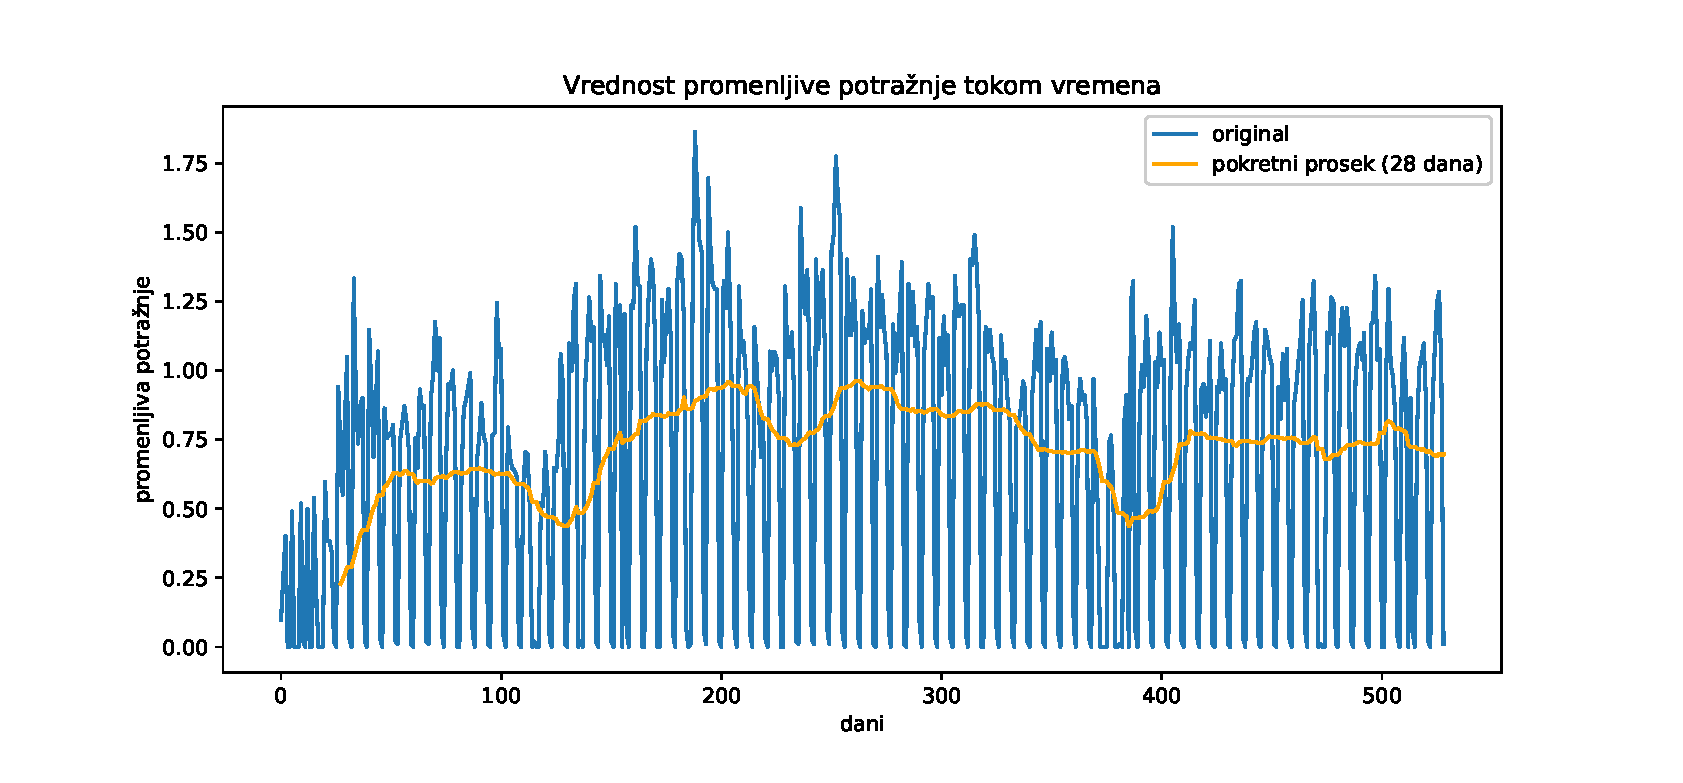
\includegraphics[width=1\textwidth]{./grafici/vremenska_serija_primer.eps}
  \caption{Primer ispitivane vremenske serije na dnevnom nivou} 
  \label{fig:vremenska_serija}
\end{figure}

\subsection{Problem posmatran kroz atribute}
Pored posmatranja problema u vidu vremenske serije, problem je posmatran i kao regresioni problem koji zavisi od nekoliko atributa koji ga opisuju. Rešavan je ansambl (\textit{eng.} ensemble) metodom, ekstremnog gradijentnog pojačavanja (\textit{eng.} XGBoost - eXtreme Gradient Boosting). Cilj je bio pronaći vezu između dostupnih atributa i ciljne promenljive koja predstavlja vrednost potražnje. Primer skupa atributa i ciljne promenljive prikazan je na slici \ref{fig:atributi}.

\section{Pregled dosadašnjih istraživanja}
Podaci korišćeni u radu dolaze iz novog izvora (pokrenut krajem 2019. godine), koji je dostupan korisnicima za rezervisanje popravki automobila, tako da su istraživanja nad ovim podacima prilično mlada i nisu javno dostupna. Što se tiče automobilske industrije i predviđanja potražnje vezane za popravke automobila i rezervne delove, takvih istraživanja postoji nekoliko. U radu \cite{callegaro2010forecasting}, dat je veoma detaljan pregled različitih metoda i modela koji se koriste za predviđanja kao što su: jednostavno eksponencijalno izravnavanje (\textit{eng.} Single Exponential Smoothing), Croston-ova metoda (\textit{eng.} Croston's Method), metoda pokretnih proseka (\textit{eng.} Moving Average), autoregresivni model pokretnih proseka za integrisane vremenske serije (\textit{eng.} ARIMA - Autoregressive Integrated Moving Average), neuronske mreže (\textit{eng.} neural networks), kao i detaljan tabelarni pregled autora koji su koristili neke od metoda i modela u svojim istraživanjima. U master radu \cite{henkelmann2018deep}, prikazan je opširan pristup predviđanju potražnje automobilskih rezervnih delova dubokim učenjem. Rad \cite{zunic2020application} se bavi predviđanjem prodaje proizvoda u maloprodajnoj industriji nad realnim podacima, korišćenjem Prophet alata za predviđanje kod vremenskih serija. U radu \cite{saravanan2019forecasting} je predstavljeno predviđanje prodaje rezervnih delova ARIMA metodom. Navedeni pregled istraživanja potvrđuje koliko je problem predviđanja potražnje zastupljen u svakodnevnom svetu i pokazuje širinu isprobanih metoda koje mogu biti iskorišćene za rešavanje problema. Neke od navedenih metoda su analizirane kroz ovaj rad.

% % primer referisanja na poglavlja i strane poglavlja
% Više detalja biće dato u glavi \ref{chp:razrada} na strani \pageref{chp:razrada}.
% ------------------------------------------------------------------------------
\chapter{Opis korišćenih metoda i metrika}
\label{chp:metode}
U ovom poglavlju biće dat kratak pregled korišćenih metoda za rešavanje definisanog problema predviđanja potražnje u industriji popravke automobila. Te metode su: 
\begin{enumerate}
    \item ARIMA,
    \item Prophet,
    \item XGBoost.
\end{enumerate}
Pored korišćenih metoda, ukratko će biti opisane i metrike za evaluaciju modela i nekoliko pojmova značajnih za rad.

\section{ARIMA}
ARIMA predstavlja algoritam za predviđanje ciljne promenljive kod vremenskih serija. Ona je dizajnirana da identifikuje obrasce u potražnji koja se desila i obrasce koji se ponavljaju kroz vreme \cite{moon2018demand}. ARIMA posmatrana u radu predstavlja model jednostavne (univarijantne) vremenske serije, gde je predviđanje zasnovano isključivo na prethodnim vrednostima. Ovaj metod objašnjava promene u vremenskoj seriji kroz tri parametra: (p, d, q). 

Prvi parametar (p), predstavlja red autoregresivne komponente modela AR(p). Autoregresivna komponenta predstavlja vezu (linearnu regresiju) između trenutne vrednosti vremenske serije i njenih prethodnih p-vrednosti, sa parametrima koji predstavljaju težine uticaja prethodnih vrednosti na trenutnu vrednost. AR(p) model se može predstaviti jednačinom: 
$$ y_t = \phi_1y_{t-1} + \phi_2y_{t-2} + \dots + \phi_py_{t-p} + \epsilon_t,$$ gde je $\epsilon_t$ beli šum/greška (\textit{eng.} white noise), $\phi_i$ su koeficijenti AR parametara, $y_t$ je vrednost serije u vremenu t, \textit{p} je broj prethodnih merenja koja se uzimaju u obzir.
% $\delta$ je predstavljeno jednačinom:
% $$ \delta = (1 - \phi_1 - \phi_2 - \dots - \phi_p)\mu, $$ gde $\mu$ predstavlja prosek promenljive y.\\
Drugi parametar (d), predstavlja red operacije diferenciranja I(d) primenjene d puta na vremensku seriju, sa ciljem da serija postane stacionarna\footnote{Vremenska serija je stacionarna kada sve njene vrednosti odgovaraju istoj raspodeli verovatnoće, nevezano za vreme \cite{vargas2017automobile}. Odnosno, kada serija nema trend ili sezonalnost i kad su statistička svojstva konstanta kroz vreme \cite{saravanan2019forecasting}.}. Diferenciranje predstavlja pojam promene između dve uzastopne posmatrane vrednosti u originalnoj seriji. Ono se može predstaviti jednačinom:
$$y'_t = y_t - y_{t-1}.$$
Ukoliko se uvede operator pomeraja \textit{B}, kao $By_t=y_{t-1}$, onda se prethodna jednačina može zapisati u obliku:
$$y'_t = y_t - y_{t-1} = y_t - By_t = (1-B)y_t.$$
Ukoliko je d=2, jednačina postaje:
$$y''_t = (y_t-y_{t-1}) - (y_{t-1}-y_{t-2}) = y_t - 2y_{t-1} + y_{t-2} = (1-2B+B^2)y_t = (1-B)^2y_t.$$
Uopšteno, operacija diferenciranja primenjena d puta se predstavlja kao: $(1-B)^{d}y_t$. 
Treći parametar (q), predstavlja red komponente pokretnih proseka (\textit{eng.} moving averages) MA(q), i pomoću nje se pravi veza između trenutne vrednosti vremenske serije i prethodnih q vrednosti greške predviđanja. MA(q) model se može predstaviti jednačinom:
$$y_t = \epsilon_t + \theta_1\epsilon_{t-1} + \theta_2\epsilon_{t-2} + \dots + \theta_q\epsilon_{t-q}, $$
gde $\theta_i$ vrednosti predstavljaju koeficijente MA parametara, \textit{q} je broj prethodnih merenja koja se uzimaju u obzir.

Procesi mogu da imaju obe komponente: AR i MA, što predstavlja ARMA proces tj. model. Kada se ukombinuju AR i MA modeli, ARMA model dobija oblik predstavljen jednačinom:
\begin{equation*}
y_t = \phi_1y_{t-1} + \phi_2y_{t-2} + \dots + \phi_py_{t-p} + \epsilon_t + \theta_1\epsilon_{t-1} + \theta_2\epsilon_{t-2} + \dots + \theta_q\epsilon_{t-q},
\end{equation*}
odnosno:
\begin{equation*}
(1-\phi_1B-\phi_2B^2-\dots-\phi_pB^p)y_t = (1+\theta_1B+\theta_2B^2+\dots+\theta_qB^q)\epsilon_t.
\end{equation*}
Uvođenjem autoregresivnog operatora: 
$$\phi(B)=1-\phi_1B-\phi_2B^2-\dots-\phi_pB^p=1-\sum\limits_{j=1}^{p}\phi_jB^j$$
i operatora pokretnih proseka:
$$\theta(B)=1+\theta_1B+\theta_2B^2+\dots+\theta_qB^q=1+\sum\limits_{j=1}^{q}\theta_jB^j,$$
ARMA(p, q) model dobija sažeti oblik:
$\phi(B)y_t = \theta(B)\epsilon_t.$
Ako u opštem slučaju diferenciranu seriju $(1-B)^dy_t$, modeliramo ARMA(p, q) procesom, tada dobijamo ARIMA(p, d, q) model:
$$\phi(B)(1-B)^dy_t = \theta_0 + \theta(B)\epsilon_t.$$
Uvedena konstanta $\theta_0$ zavisi od reda diferenciranja. Ako je proces stacionaran (d=0), onda je $\theta_0$ u relaciji sa sredinom procesa: $\theta_0=\mu(1-\phi_1-\dots-\phi_p)$ \cite{zlatko}.\\
ARIMA model može da ima i sezonske komponente: (P, D, Q), kada se nazima SARIMA. Sezonske komponente predstavljaju regularne obrasce promena koje se ponavljaju svakih S vremenskih perioda, gde je S broj vremenskih perioda dok se obrazac opet ne ponovi. Detaljnije o SARIMA modelu se može naći u \cite{hyndman2018forecasting}.

\section{Prophet}
Prophet je alat za predviđanje ciljne promenljive kod vremenskih serija. Razvijen je od strane Facebook zajednice \cite{prophet} i može da generiše prognoze razumnog kvaliteta. Alat je otvorenog tipa (\textit{eng.} open-source) i zasnovan je na aditivnom modelu, gde se nelinearni trendovi aproksimiraju godišnjom, nedeljnom i dnevnom sezonalnošću. Ono što Prophet ima kao opciju je uključivanje efekta praznika u model. Robustan je na nedostajuće vrednosti i promene u trendu, i tipično dobro obrađuje vrednosti van granica (\textit{eng.} outliers) \cite{zunic2020application}.

U originalnom radu u kome autori predstavljaju Prophet \cite{taylor2018forecasting}, pomenuti model je predstavljen jednačinom:
\begin{equation*}
\label{eq: prophet}
y(t) = g(t) + s(t) + h(t) + \epsilon_t,
\end{equation*}
gde $g(t)$ predstavlja funkciju trenda koja modeluje neperiodične promene vrednosti ciljne promenljive, $s(t)$ predstavlja periodične promene (npr. sezonalne promene dnevnog ili godišnjeg nivoa), $h(t)$ predstavlja efekat praznika koji mogu da se javljaju u neregularnim trenucima i da traju jedan ili više dana, $\epsilon_t$ se odnosi na grešku i obuhvata sve promene koje nisu obuhvaćene modelom. Greške treba da imaju normalnu raspodelu i da su nezavisne, jednako raspoređene veličine (beli šum). Pored navedenih opcija, moguće je kreirati sopstveni sezonalni efekat (npr. mesečni) koji se formira korišćenjem parcijalne Furijeove sume\footnote{Više se može pročitati na \url{https://facebook.github.io/prophet/}}. Prophet ima podršku za programski jezik Python i programski jezik R.

\section{XGBoost}
Osnovna ideja metoda pojačavanja je da se ansambl izgradi dodavanjem jednog po jednog modela, gde svaki model uči tako da što bolje nadomesti mane trenutnog skupa modela \cite{ml}. AdaBoost je bitan, poznatiji algoritam pojačavanja i radi po principu uvećavanja težina instanci koje su pogrešno klasifikovane, pa se sledeći model fokusira na te instance kako bi se celokupno stanje poboljšalo \cite{mayr2014evolution}. Instanca u ovom slučaju predstavlja par vrednosti $(x_i, y_i)$, gde su sa $x_i$ predstavljene vrednosti atributa koje opisuju vrednost ciljne promenljive $y_i$.

Osim pojačavanja, postoje i gradijentna pojačavanja i ona su po pitanju preciznosti među najboljim metodama mašinskog učenja. Osnovna ideja ovih metoda dolazi iz gradijentnih optimizacionih metoda, gde se tekuće rešenje popravlja dodavanjem vektora proporcionalnog negativnoj vrednosti gradijenta funkcije koja se minimizuje \cite{ml}. 

Ekstremno gradijentno pojačavanje (XGBoost), predstavlja ansambl sistem pojačavanja zasnovan na stablima odlučivanja. Evolucija algoritama je predstavljena na slici \ref{fig: xgboost_evolucija} i može se videti da je regularizacija jedna od novina kod XGBoost metode.
\begin{figure}[!ht]
  \centering
  \captionsetup{justification=centering}
  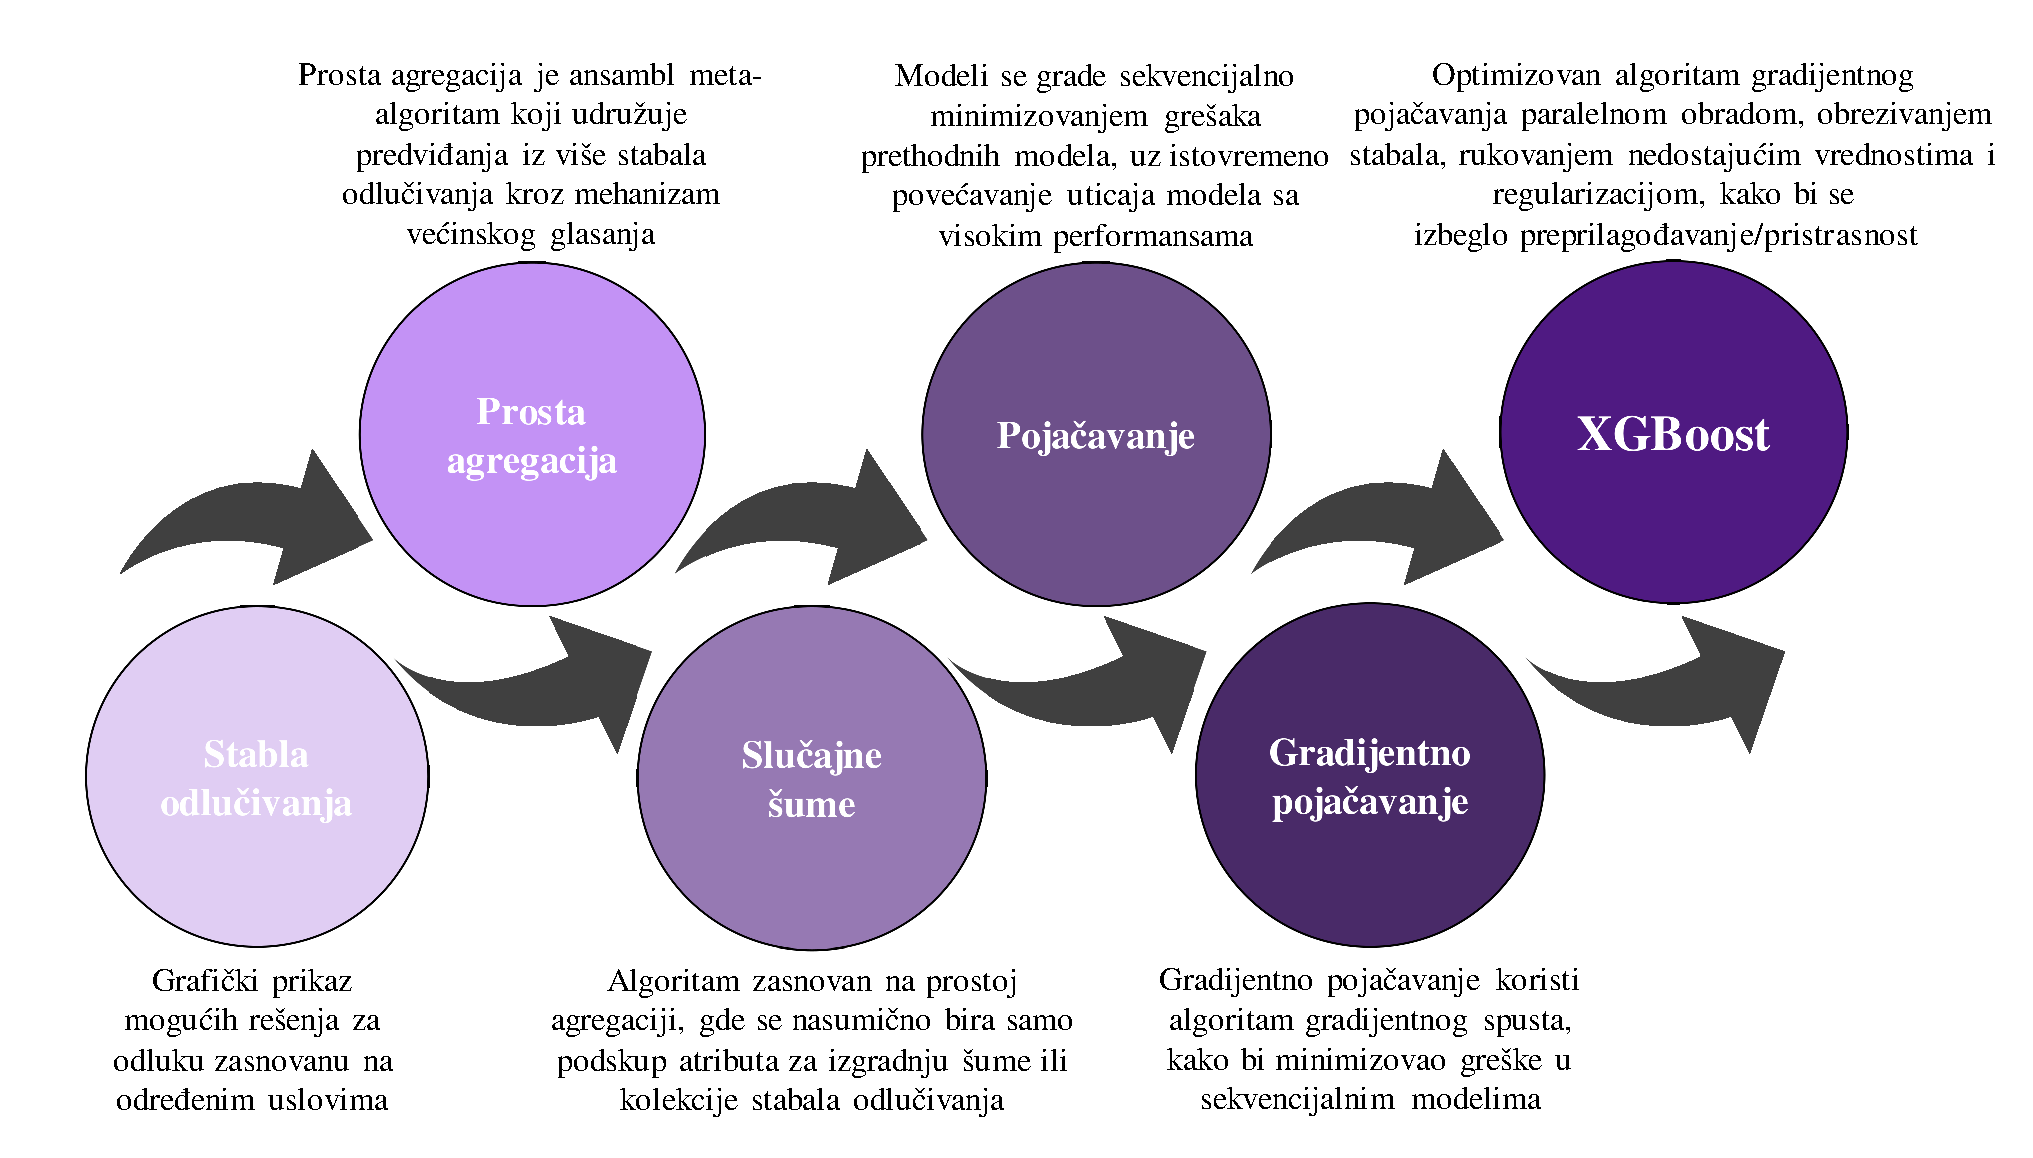
\includegraphics[width=1\textwidth]{./grafici/xgboost_evolucija_prevod.eps}
  \caption{Evolucija XGBoost algoritma od stabala odlučivanja}
  \vspace{-10pt}
  \caption*{\tiny{Prevod slike iz izvora na lokaciji: \url{https://towardsdatascience.com/https-medium-com-vishalmorde-xgboost-algorithm-long-she-may-rein-edd9f99be63d}}}
  \label{fig: xgboost_evolucija}
\end{figure}
Sam algoritam je poznat po svojoj skalabilnosti, dobrom ponašanju sa retkim (\textit{eng.} sparse) podacima, distribuiranosti i takođe je podržan od strane nekoliko programskih jezika, među kojima je i Python \cite{chen2016xgboost}.

\section{Metrike}
Kroz rad je ispraćeno nekoliko metrika za evaluaciju modela. Korišćene metrike su:
\begin{itemize}
    \item Srednja apsolutna greška (MAE),
    \item Srednje kvadratna greška (MSE),
    \item Kvadratni koren srednje kvadratne greške (RMSE),
    \item Simetrična srednja apsolutna procentualna greška (SMAPE).
\end{itemize}
Ključna metrika koja je praćena je SMAPE, ali i ostale metrike su propraćene kroz modele. U nastavku će biti detaljnije opisana SMAPE metrika.

\subsection{Prilagođena SMAPE metrika} 
SMAPE (\textit{eng.} Symmetric Mean Average Percentage Error) metrika je prilagođena za potrebe projekta na sledeći način:
\begin{equation*}
\frac{\sum\limits_{t=1}^{N} |F_t - A_t|} {\sum\limits_{t=1}^{N}max(A_t, F_t)}\text{,}
\end{equation*}
dok je originalna formula za SMAPE metriku: 
\begin{equation*}
\frac{\sum\limits_{t=1}^{N} |F_t - A_t|} {\sum\limits_{t=1}^{N}(A_t + F_t)}\text{.}
\end{equation*}
U formuli $F_t$ predstavlja predviđenu vrednost u vremenu $t$, $A_t$ predstavlja stvarnu vrednost u vremenu $t$, a $N$ je broj instanci tj. uzoraka modela.
Razlog za izmenu originalne metrike je taj što u situaciji kada model potcenjuje, greška je značajno razumljivija za tumačenje. Na primer, u situaciji kada je stvarna vrednost $100$, a predviđena vrednost $50$, originalna SMAPE metrika daje vrednost $0.33$, dok prilagođena SMAPE metrika daje vrednost $0.5$. Čak i u situaciji kada se javlja precenjivanje, recimo predviđena vrednost je $150$, za već pomenutu stvarnu vrednost, prilagođena SMAPE metrika daje vrednost $0.33$, dok je originalna SMAPE metrika $0.2$ -- što ima više smisla pri tumačenju rezultata od strane radnika koji planiraju sezonu. \\
\newline
Osim metrika za evaluaciju modela, korišćena je AIC metrika (\textit{Akaike Information Criterion}\footnote{\url{https://en.wikipedia.org/wiki/Akaike_information_criterion}}), za evaluaciju ARIMA modela kod vremenskih serija. Manja vrednost ove metrike označava bolji model.

\section{Kodiranje uticajem}
\label{lbl: impact_encoding}
Kodiranje uticajem (\textit{eng.} Impact Encoding), predstavlja jednu vrstu kodiranja kategoričkih atributa u redne vrednosti. Ono predstavlja nadogradnju na ciljno kodiranje (\textit{eng.} Target Encoding) \cite{pargent2019benchmark} i praktičnije je od binarizacije atributa zbog toga što dodaje samo jednu kolonu koja predstavlja izlaz, za razliku od binarizacije atributa gde se dodaje nova kolona za svaku različitu vrednost atributa. Kodiranje uticajem se sastoji od tri koraka: ciljnog kodiranja, regularizacije i normalizacije.

Ciljno kodiranje je deo koji svaku vrednost kategoričkog atributa zamenjuje prosečnom vrednošću koju baš ta vrednost kategoričkog atributa ima u koloni ciljne promenljive. Recimo, ako je kategorički atribut boja i ona može da uzme vrednosti: crvena i plava, onda crvenu kodiramo sa prosekom vrednosti koju crvena ima u koloni ciljne promenljive. Ovo se može zapisati sledećom formulom u kojoj $T_{c_v}$ predstavlja vrednost kategoričkog atributa $c_v$ u koloni ciljne promenljive: 

\begin{center}
$c_v \to \frac{\sum\limits_{i=1}^{N}{T_{c_v}}}{|c_v|}.$ 
\end{center}
Konkretnije, u tabeli \ref{tbl: kodiranje_uticajem} je dat primer skupa podataka sa jednim atributom koji je kategorički i sa numeričkom ciljnom promenljivom $T$. 
\begin{table}
\centering
\caption{Primer skupa podataka za ciljno kodiranje}
\label{tbl: kodiranje_uticajem}
\begin{tabular}{ |c|c|} 
\hline
BOJA & T \\
\hline
crvena & 2.5 \\
plava & 2.0 \\
plava & 0.5 \\
crvena & 1.8 \\
\hline
\end{tabular}
\end{table}
Primenom ciljnog kodiranja na atribut $BOJA$, svuda gde se javlja vrednost $crvena$ će biti dodeljena vrednost $\frac{(2.5 + 1.8)}{2}$, jer su $2.5$ i $1.8$ vrednosti u koloni $T$, a ukupan broj redova u kojima se javlja vrednost $crvena$ je $2$, pa se zato deli tim brojem. Na isti način vrednost $plava$ se svuda zamenjuje sa $\frac{(2.0 + 0.5)}{2}$.\\
Deo regularizacije kodiranja se bavi problemom da ne verujemo baš svakom zamenjivanju vrednosti jednako. Ovaj problem se javlja u praksi kada vrednost ciljne promenljive za jednu vrednost kategoričkog atributa može da bude ogromna, a da te vrednosti atributa ima jako malo; naspram puno vrednosti kategoričkog atributa čije su vrednosti koje odgovaraju ciljnoj promenljivoj dosta manje. Želimo da izbalansiramo ovu situaciju i to se rešava uvođenjem parametra $\alpha := \max |c_v|$, koji predstavlja maksimum broja pojavljivanja različitih vrednosti posmatranog kategoričkog atributa. Tada kodiranje postaje prebacivanje atributa u vrednost: 
$$c_v \to \frac{|c_v|\mu_{T_{c_v}} + \alpha\mu_{T}}{|c_v| + \alpha},$$
gde $\mu_{T_{c_v}}$ predstavlja prosek vrednosti ciljne promenljive koje odgovaraju $c_v$ vrednosti razmatranog kategoričkog atributa $c$, a $\mu_T$ predstavlja globalni prosek svih vrednosti ciljne promenljive.\\
Deo normalizacije rešava problem kada kodiranje uticajem radimo nad trening podacima, a u test skup nam dođe vrednost atributa koja nije viđena u trening skupu dok smo vršili prebacivanje vrednosti. Rešenje u ovoj situaciji je normiranje svakog od dobijenih uticaja različitih vrednosti atributa (na prethodno opisan način), prosekom svih dobijenih uticaja za taj kategorički atribut:
\begin{center}
$c_v \to \frac{\frac{|c_v|\mu_{T_{c_v}} + \alpha\mu_{T}}{|c_v| + \alpha}}{\mu_{c}}$.
\end{center}
Na ovaj način, nepoznatim instancama može da se dodeli vrednost 1, koja implicira da je uticaj očekivana srednja vrednost svih klasa (različitih vrednosti atributa) i da nema odstupanja od populacije.

% ------------------------------------------------------------------------------

% ------------------------------------------------------------------------------
\chapter{Prikaz rada metoda i rezultati}

\section{Podaci}
Podaci korišćeni u radu su prikupljeni od jedne Švedske kompanije. Predstavljaju realne podatke iz industrije, a važno je napomenuti da su dobijeni sa samo jednog izvora koji je dostupan njihovim korisnicima. Radi se o novom načinu rezervisanja popravki automobila na različitim lokacijama, putem interneta (\textit{eng.} booking portal). Portal je krenuo sa radom krajem 2019. godine, tako da količina dostupnih podataka nije velika. Takođe, zbog pandemije Covid19 količina dostupnih podataka je ograničena i ovo istraživanje nad njima možda bude od posebnog značaja u budućnosti, pre svega kada pomenuti portal za rezervacije bude izvor veće količine informacija.

Podaci se sastoje od informacija kao što su: koja marka automobila je došla u koju registrovanu automehaničarsku radnju, kog datuma i od propratnih informacija vezanih za popravku. Primer skupa atributa i ciljne promenljive je prikazan na slici \ref{fig:atributi}.
\begin{figure}[!ht]
  \centering
  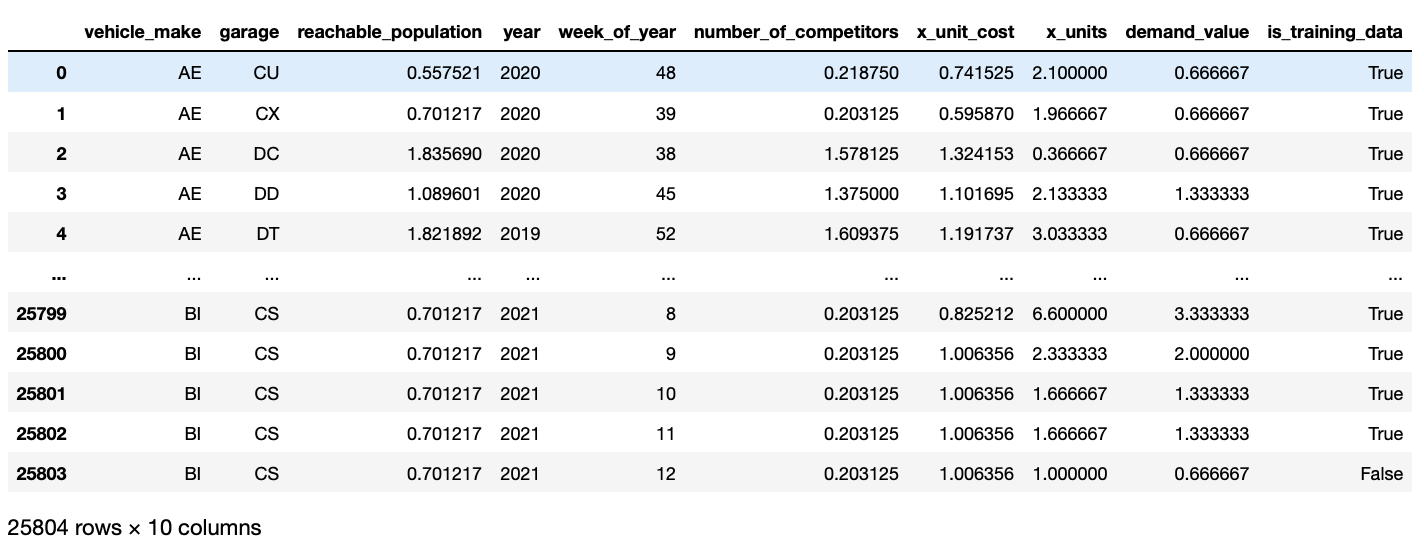
\includegraphics[width=1\textwidth]{./grafici/atributi_primer.png}
  \caption{Primer skupa atributa i ciljne promenljive iz rada}    
  \label{fig:atributi}
\end{figure}
Svi korišćeni kategorički atributi su morali biti šifrovani kombinacijama slova zbog privatnosti firme, a svi numerički atributi su normirani. Na slici \ref{fig:atributi} je predstavljen primer skupa podataka za predviđanje promenljive \textit{demand\_value} na nedeljnom nivou, u kome su podaci grupisani po markama automobila i automehaničarskim radnjama. Atributi \textit{x\_units} i \textit{x\_unit\_cost} su vezani za informacije o konkretnim rezervacijama, od kojih u modelima nije korišćen \textit{x\_units}, kako ne bi dolazilo do potencijalnog curenja informacija u modelu. Atribut \textit{x\_unit\_cost} predstavlja cenu usluge koja je vezana za konkretnu radnju i automobil.

\subsection{Obogaćivanje podataka eksternim podacima}
Atributi broj konkurenata (\textit{number\_of\_competitors}) i dostižno stanovništvo (\textit{reachable\_population}), su generisani na osnovu firminih informacija o lokacijama automehaničarskih radnji. Za svaku radnju su poznate geografska širina i geografska dužina. Atribut \textit{reachable\_population} je kreiran od strane zaposlenih u firmi, na osnovu javnih statističkih podataka o populaciji stanovništva u regionima radnji. On predstavlja sumu populacije velikih regiona u opsegu koji predstavlja rastojanje pređeno za 40 minuta vožnje, brzinom 60 km/h, od lokacije radnje. 

Atribut \textit{number\_of\_competitors} je dodat u sklopu ovog rada. On predstavlja broj drugih radnji (konkurenata) u opsegu od 80km od automehaničarske radnje. Vrednost od 80km je uzeta kao neka racionalna vrednost za voženje do neke jeftinije radnje ili do radnje koja nije u drugom gradu. Vrednost ovog atributa je kreirana korišćenjem Open Street Map (OSM)\footnote{\url{https://www.openstreetmap.org}}, odnosno besplatne mape sveta. OSM ima besplatan servis za dohvatanje raznih informacija na osnovu zadatih parametara, korišćenjem njihovog upitnog jezika. Servis se zove Overpass API\footnote{\url{https://overpass-turbo.eu}} i zadavanjem lokacija radnji i specijalne oznake (taga) \textbf{\textit{'shop'='car\_repair'}}, dobijene su informacije o radnjama u okolini, u \textit{json} formatu. Primer kôda koji je korišćen za dohvatanje informacija o radnjama je prikazan u listingu \ref{lbl: overpass_funkcija}.
\begin{table}
\begin{lstlisting}[language=python, belowskip=-\baselineskip, frame=single, label=lbl: overpass_funkcija, caption={Funkcija za dohvatanje informacija o drugim radnjama u okolini}]
overpass_url = "http://overpass-api.de/api/interpreter"

def overpass_query(latitude, longitude, km_around):
    overpass_query = "[out:json];(node(around:{},{},{})
                      ['shop'='car_repair'];);
                      out;".format(km_around, latitude, longitude)

    while True:
        try:
            response = requests.get(overpass_url, 
                                    params={'data': overpass_query})
            garages_around = response.json()
            return garages_around
        except:
            print("Try again...")
\end{lstlisting} 
\end{table}
% \vspace{80pt}
Primer informacija koje se dobiju upitom ka Overpass API prikazan je na slici \ref{fig: overpass}. Kao atribut skupa podataka u ovom radu, korišćena je informacija o ukupnom broju radnji u okolini. 
\vspace{40pt}
\begin{figure}[!ht]
  \centering
  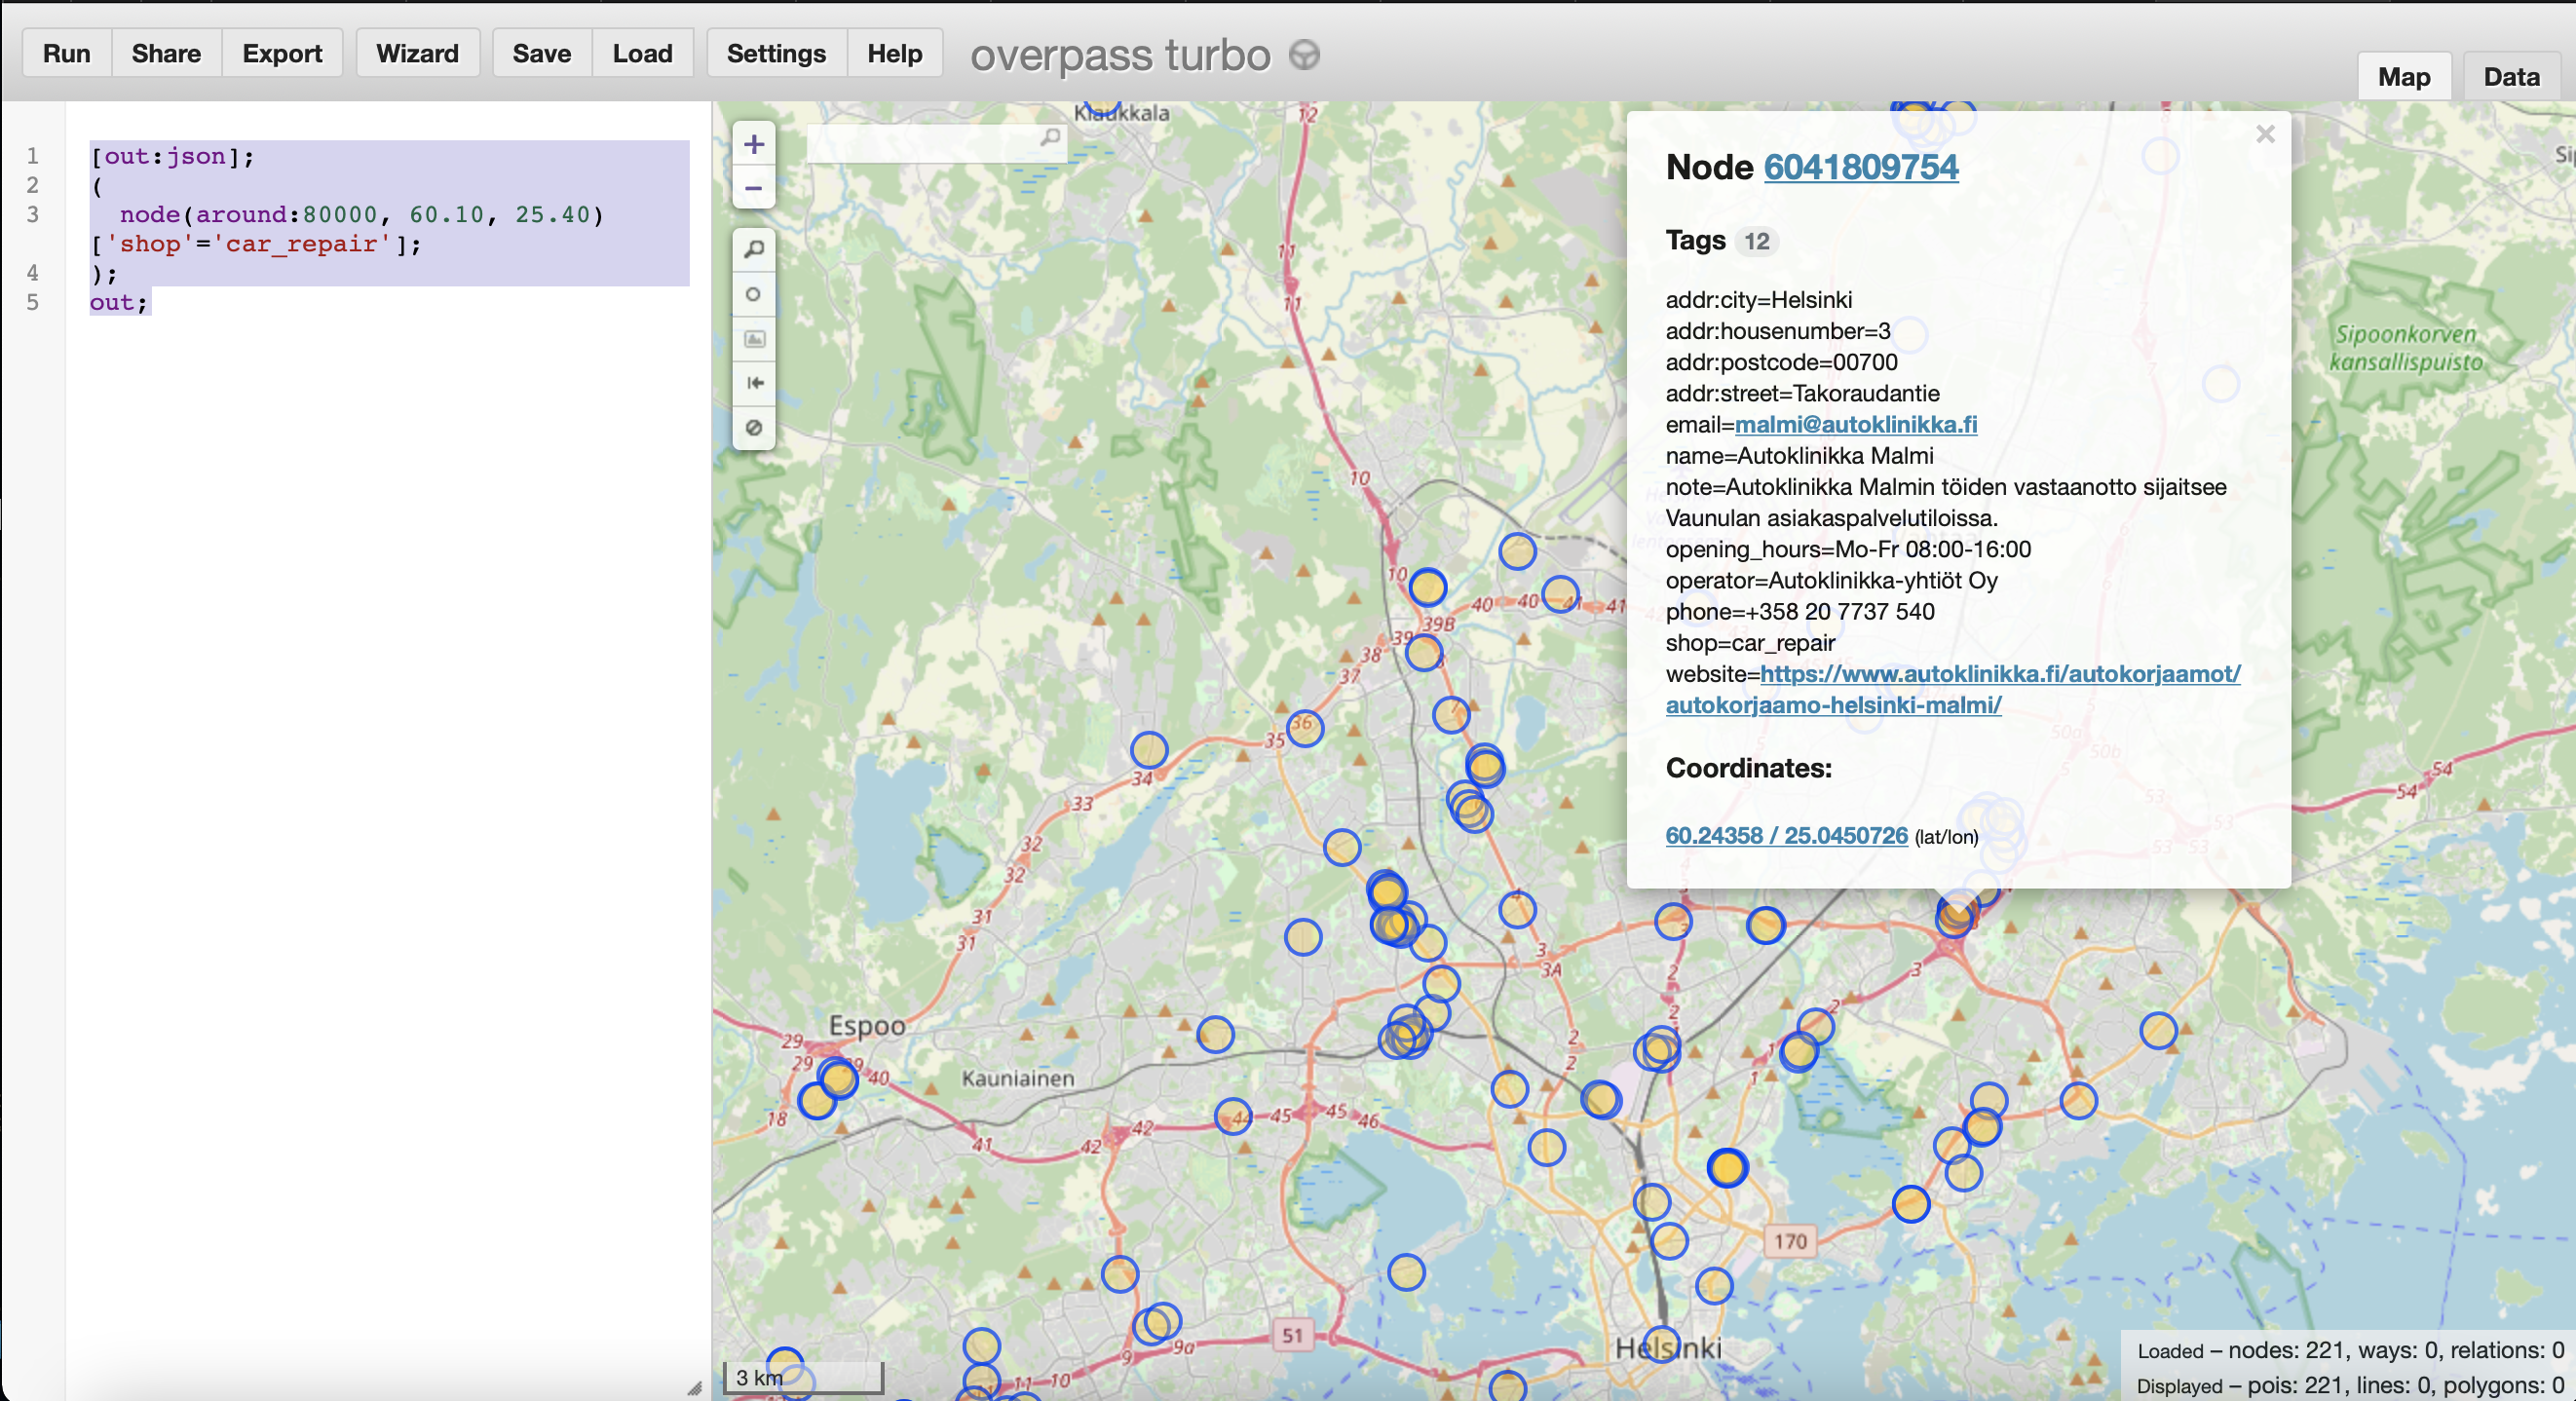
\includegraphics[width=1\textwidth]{./grafici/overpass_primer.png}
  \caption{Overpass API primer upita}
  \label{fig: overpass}
\end{figure}
\vspace{-50pt}
\subsection{}
{\parindent0pt 
Primer podataka koji je korišćen za vremenske serije na dnevnom nivou predstavljen je u tabeli \ref{tbl: daily_data_example}, a na nedeljnom nivou u tabeli \ref{tbl: weekly_data_example}. Podaci dobijeni za dnevni nivo predstavljaju grupisane i zatim sumirane vrednosti promenljive potražnje za sve automehaničarske radnje i sve marke automobila zajedno za određeni datum. Isto je urađeno i za nedeljni nivo, samo sumirano za celu nedelju. Nakon konačnog sumiranja, u oba slučaja su vrednosti normirane zbog zaštite privatnosti firme. Bitno je napomenuti da su datumi prebačeni u nedelje u godini, tako da se vodilo računa o tome da kalendarski dan bude u tekućoj kalendarskoj godini, npr. da 30.12.2019. godine bude u poslednjoj nedelji 2019. godine, a ne u prvoj nedelji 2020. godine. Odluka da tako bude je napravljena u dogovoru sa firmom, da bude usaglašena sa kalendarskom godinom i kalkulacijama na nivou godine. Primer kôda koji sređuje prebacivanje, kao i izvor sa svim podacima korišćenim u radu, dat je u Github repozitorijumu projekta na adresi: \url{https://github.com/mandja96/matf-master-rad}.
}
\begin{table}
\centering
\caption{Primer korišćenih podataka za dnevnu vremensku seriju (prvih 7 vrednosti)}
\label{tbl: daily_data_example}
\begin{tabular}{ |c|c|} 
\hline
date & demand\_value \\
\hline
2019-12-18 & 0.098\\
2019-12-19 & 0.245\\
2019-12-20 & 0.402\\
2019-12-23 & 0.490\\
2019-12-27 & 0.520\\
2019-12-28 & 0.020\\
2019-12-30 & 0.500\\
\hline
\end{tabular}
\end{table}

\begin{table}
\centering
\caption{Primer korišćenih podataka za nedeljnu vremensku seriju (prvih 7 vrednosti)}
\label{tbl: weekly_data_example}
\begin{tabular}{ |c|c|} 
\hline
year\_week & demand\_value \\
\hline
201951 & 0.144\\
201952 & 0.295\\
202001 & 0.140\\
202002 & 0.333\\
202003 & 0.790\\
202004 & 0.921\\
202005 & 0.915\\
\hline
\end{tabular}
\end{table}

\section{Dnevni nivo - na nivou države} 
U ovom poglavlju biće predstavljeni propratni koraci i dobijeni rezultati nad dnevnim podacima, koji predstavljaju jednostavnu (univarijantnu) vremensku seriju. Podaci su grupisani po datumima, za nivo cele države. Biće izložena tri opisana pristupa: ARIMA, Prophet i XGBoost. Razlog posmatranja vremenske serije nad grupisanim podacima je pre svega da se isproba ponašanje metoda, ali i da se upoznaju podaci i generalni nedostatak podataka za vremensku seriju nad zasebnim radnjama i markama (većim granularnostima -- manjoj grupaciji).

\subsubsection{Pretprocesiranje dnevnih podataka}
Pre svega je ispitano koliko datuma nedostaje u vremenskoj seriji u vremenskom periodu 18.12.2019 - 29.05.2021. Broj nedostajućih dana je 96 (manje od $20\%$ podataka) i ti dani su popunjeni vrednošću nula. Raspodela nedostajućih dana po danima nedelje je prikazana na histogramu \ref{fig: dani_nedelje}. 
% \begin{figure}[!ht]
%   \centering
%   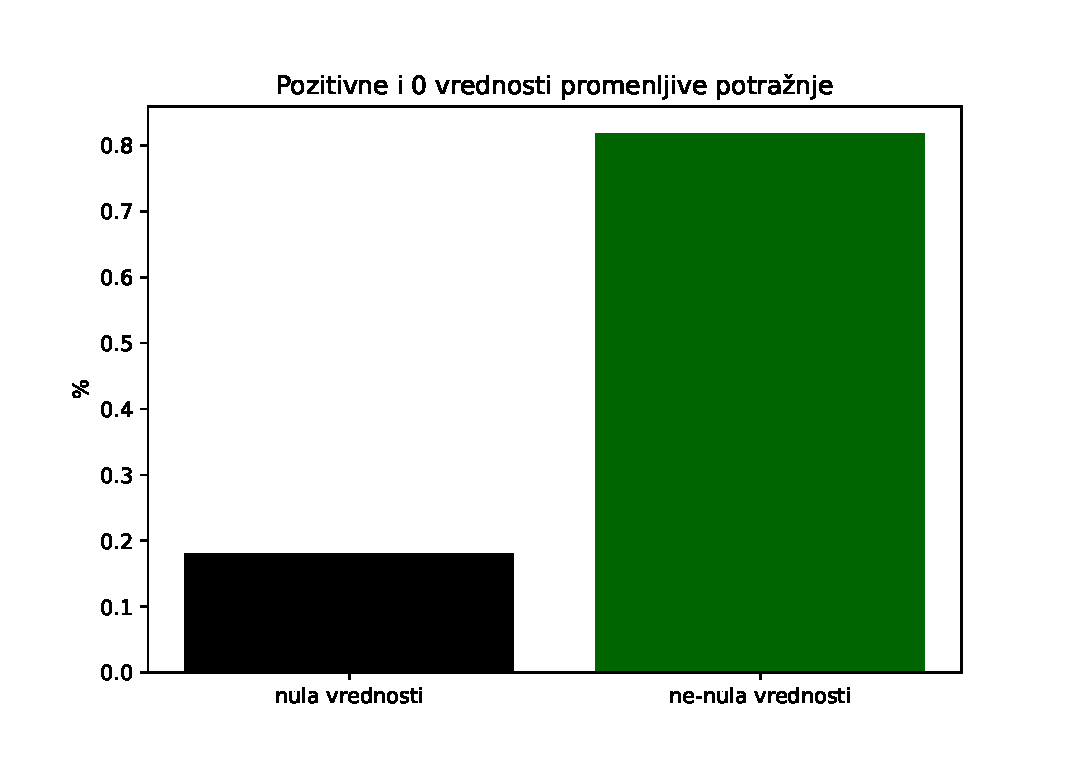
\includegraphics[width=0.8\textwidth]{./grafici/nula_vrednosti_dnevni_podaci.eps}
%   \caption{Procenat pozitivnih i nula vrednosti promenljive potražnje, nakon popunjavanja nedostajućih datuma.}
%   \label{fig: nula_nenula}
% \end{figure}
\begin{figure}[!ht]
  \centering
  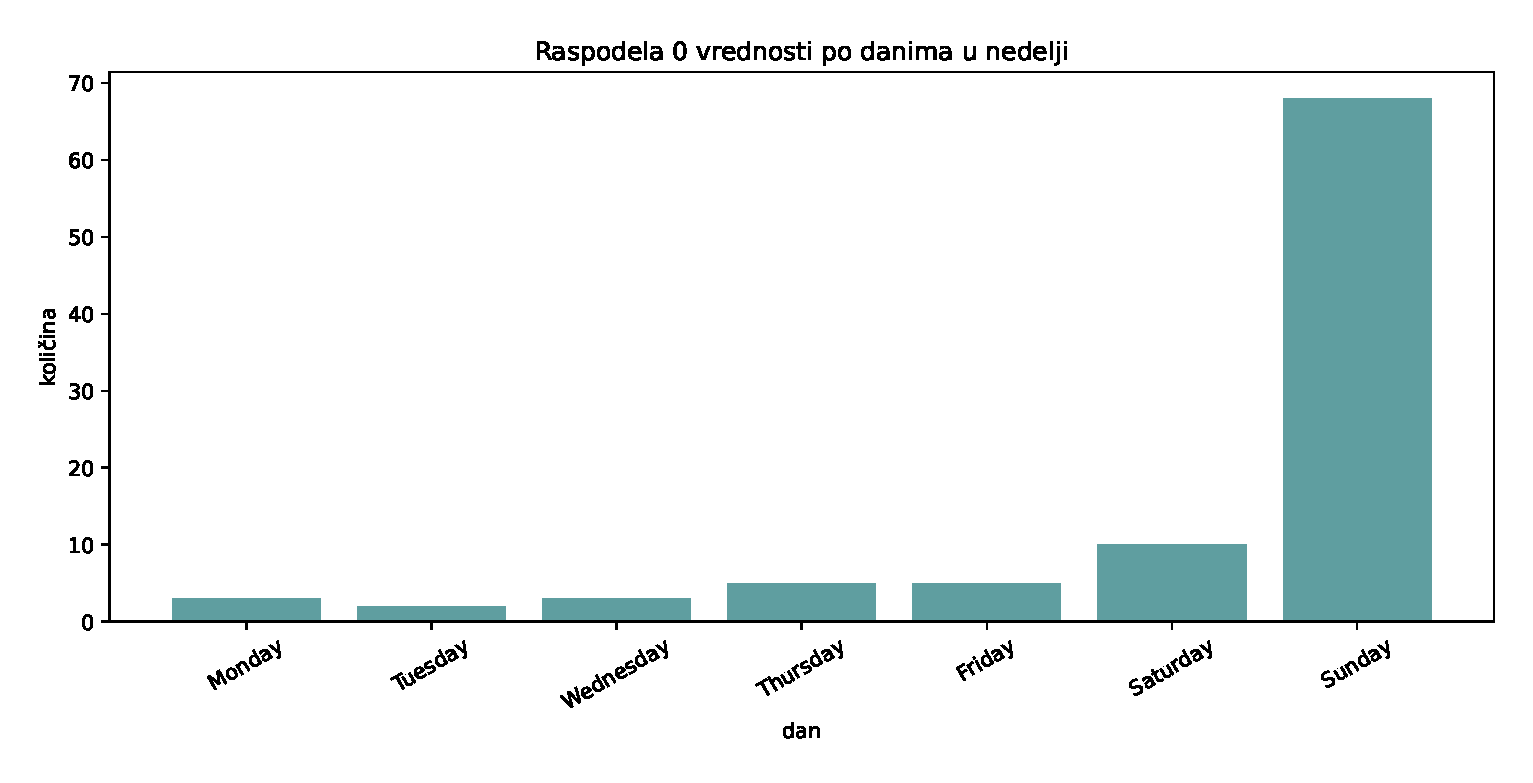
\includegraphics[width=1\textwidth]{./grafici/nule_po_danima_nedelje.eps}
  \caption{Raspodela nula vrednosti promenljive potražnje po danima u nedelji}
  \label{fig: dani_nedelje}
\end{figure}
Kao što se može videti sa histograma, većina nula vrednosti pripada nedeljama, koje predstavljaju za većinu radnji neradan dan. Ostatak datuma koji imaju vrednost nula su pretežno neki praznici koji su takođe neradni dani (oko Nove godine, Uskrsa, državnog praznika). Zbog velike zastupljenosti nula vrednosti kod nedelje kao dana u sedmici, sve nedelje su izbačene iz vremenske serije i serija je posmatrana kao da postoji šest dana u sedmici. Veličina posmatranih dana je nakon toga postala 454.

\subsection{ARIMA}
Kod ARIMA modela je bilo bitno ispitati neka svojstva vremenske serije kao što su nedostajuće vrednosti (datumi koji fale), stacionarnost, sezonalnost. Takođe, bilo je bitno ispitati grafik autokorelacione funkcije -- ACF (\textit{eng.} Auto-Correlation Function) i grafik parcijalne autokorelacione funkcije -- PACF (\textit{eng.} Partial Auto-Correlation Function), kako bi se odredili parametri (p, d, q) koji konstruišu model, ali ispitati i kako se ponaša sezonski ARIMA model (SARIMA) nad podacima. Pre gore pomenutog pretprocesiranja podataka, vremenska serija ima izgled prikazan na grafiku \ref{fig: dnevna_sa_nedeljama}, a nakon pretprocesiranja vremenska serija ima izgled prikazan na grafiku \ref{fig: dnevna_vremenska_serija_bez_nedelja}. 

\begin{figure}[!ht]
  \centering
  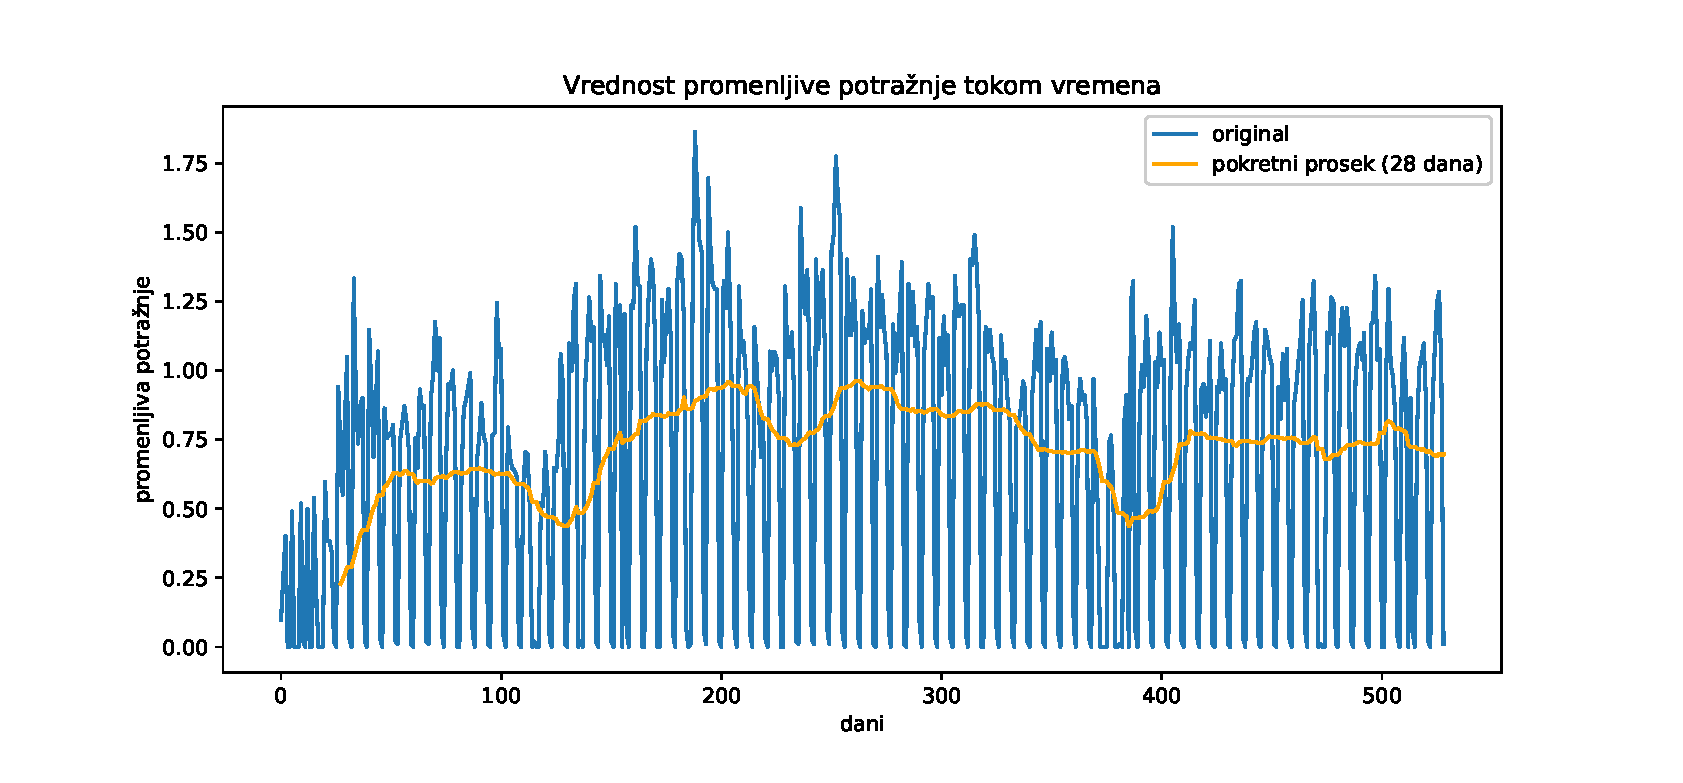
\includegraphics[width=1\textwidth]{./grafici/vremenska_serija_primer.eps}
  \caption{Vremenska serija sa nedeljama}
  \label{fig: dnevna_sa_nedeljama}
\end{figure}

\begin{figure}[!ht]
  \centering
  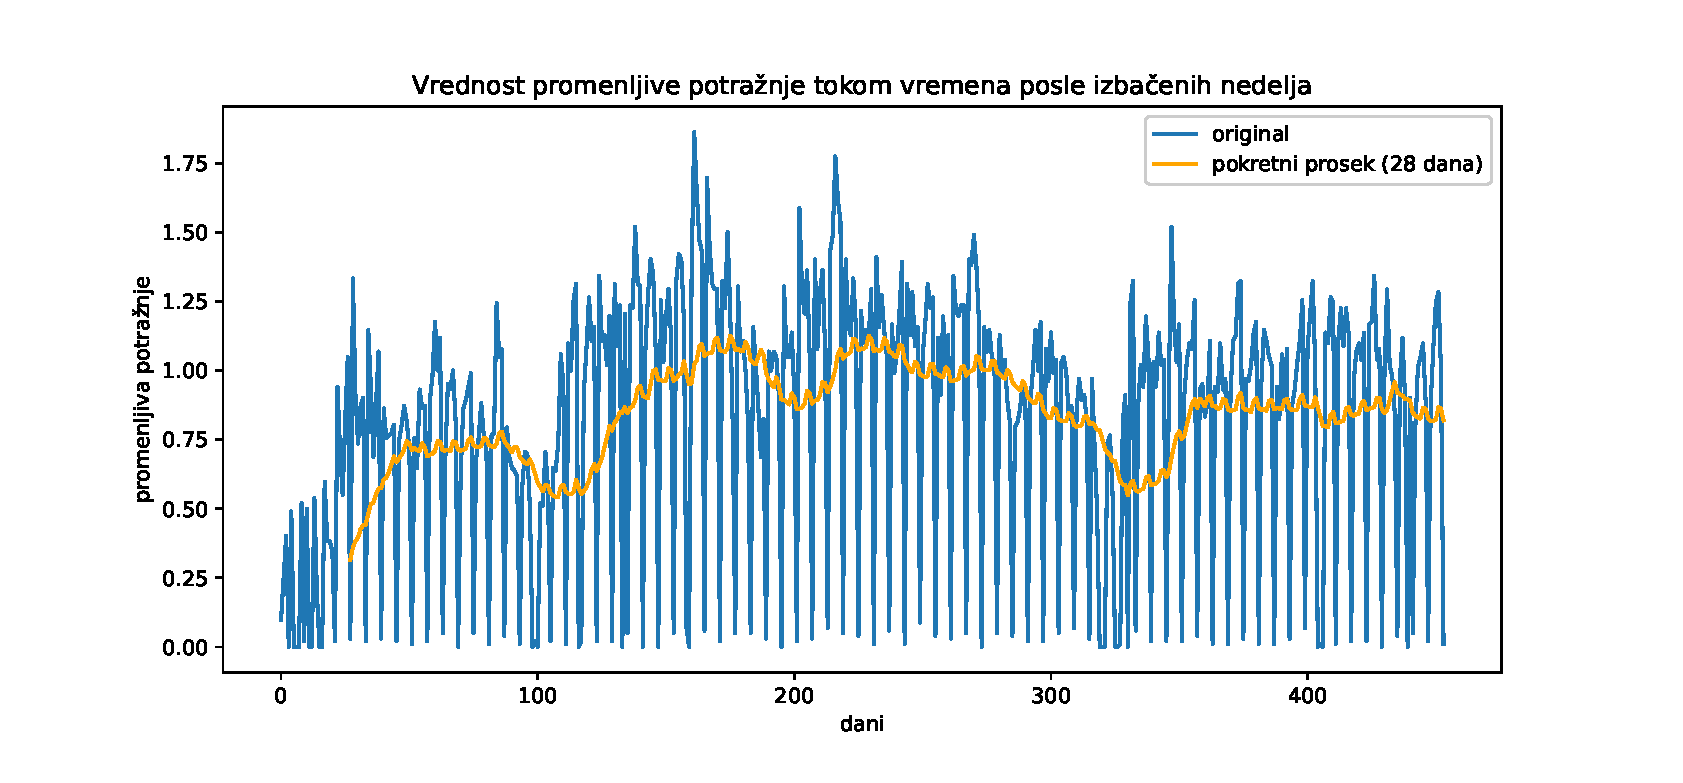
\includegraphics[width=1\textwidth]{./grafici/vremenska_serija_primer_bez_nedelja.eps}
  \caption{Vremenska serija bez nedelja}
  \label{fig: dnevna_vremenska_serija_bez_nedelja}
\end{figure}
Nakon toga, izvršeno je ispitivanje stacionarnosti serije, jer je na osnovu toga doneta odluka da li seriju treba diferencirati ili ne. U ove svrhe korišćen je statistički test stacionarnosti pod nazivom: uvećan Diki-Fuler test (\textit{eng.} Augmented Dickey-Fuller). Vrednost testa nad dnevnim podacima bez nedelja je vratila vrednosti:
\begin{minipage}{\linewidth}
\begin{verbatim}
Test Statistics                 -3.674781
p-value                          0.004482
No. of lags used                18.000000
Number of observations used    435.000000
critical value (1%)             -3.445473
critical value (5%)             -2.868207
critical value (10%)            -2.570321
\end{verbatim}
\vspace{10pt}
\end{minipage}
S obzirom da je p-vrednost manja od $0.05$, nulta hipoteza se može odbaciti, što nam govori da je serija stacionarna i da nema potrebe za diferenciranjem.

Zatim je ispitano koje vrednosti parametri p i q mogu potencijalno da imaju. Za ispitivanje ovih parametara nam pomažu ACF i PACF grafici, koji su za korišćene podatke predstavljeni na grafiku \ref{fig: acf_pacf_dnevni}. Primećujemo da originalni podaci imaju periodičan špic na svakih šest vrednosti pomeraja. To nam govori da postoji neka vrsta sezonalnosti u seriji, tako da su propraćeni i ACF/PACF grafici sa razlikom trenutne vrednosti i vrednosti u trenutku šest vrednosti u prošlosti.
\begin{figure}[!ht]
  \centering
  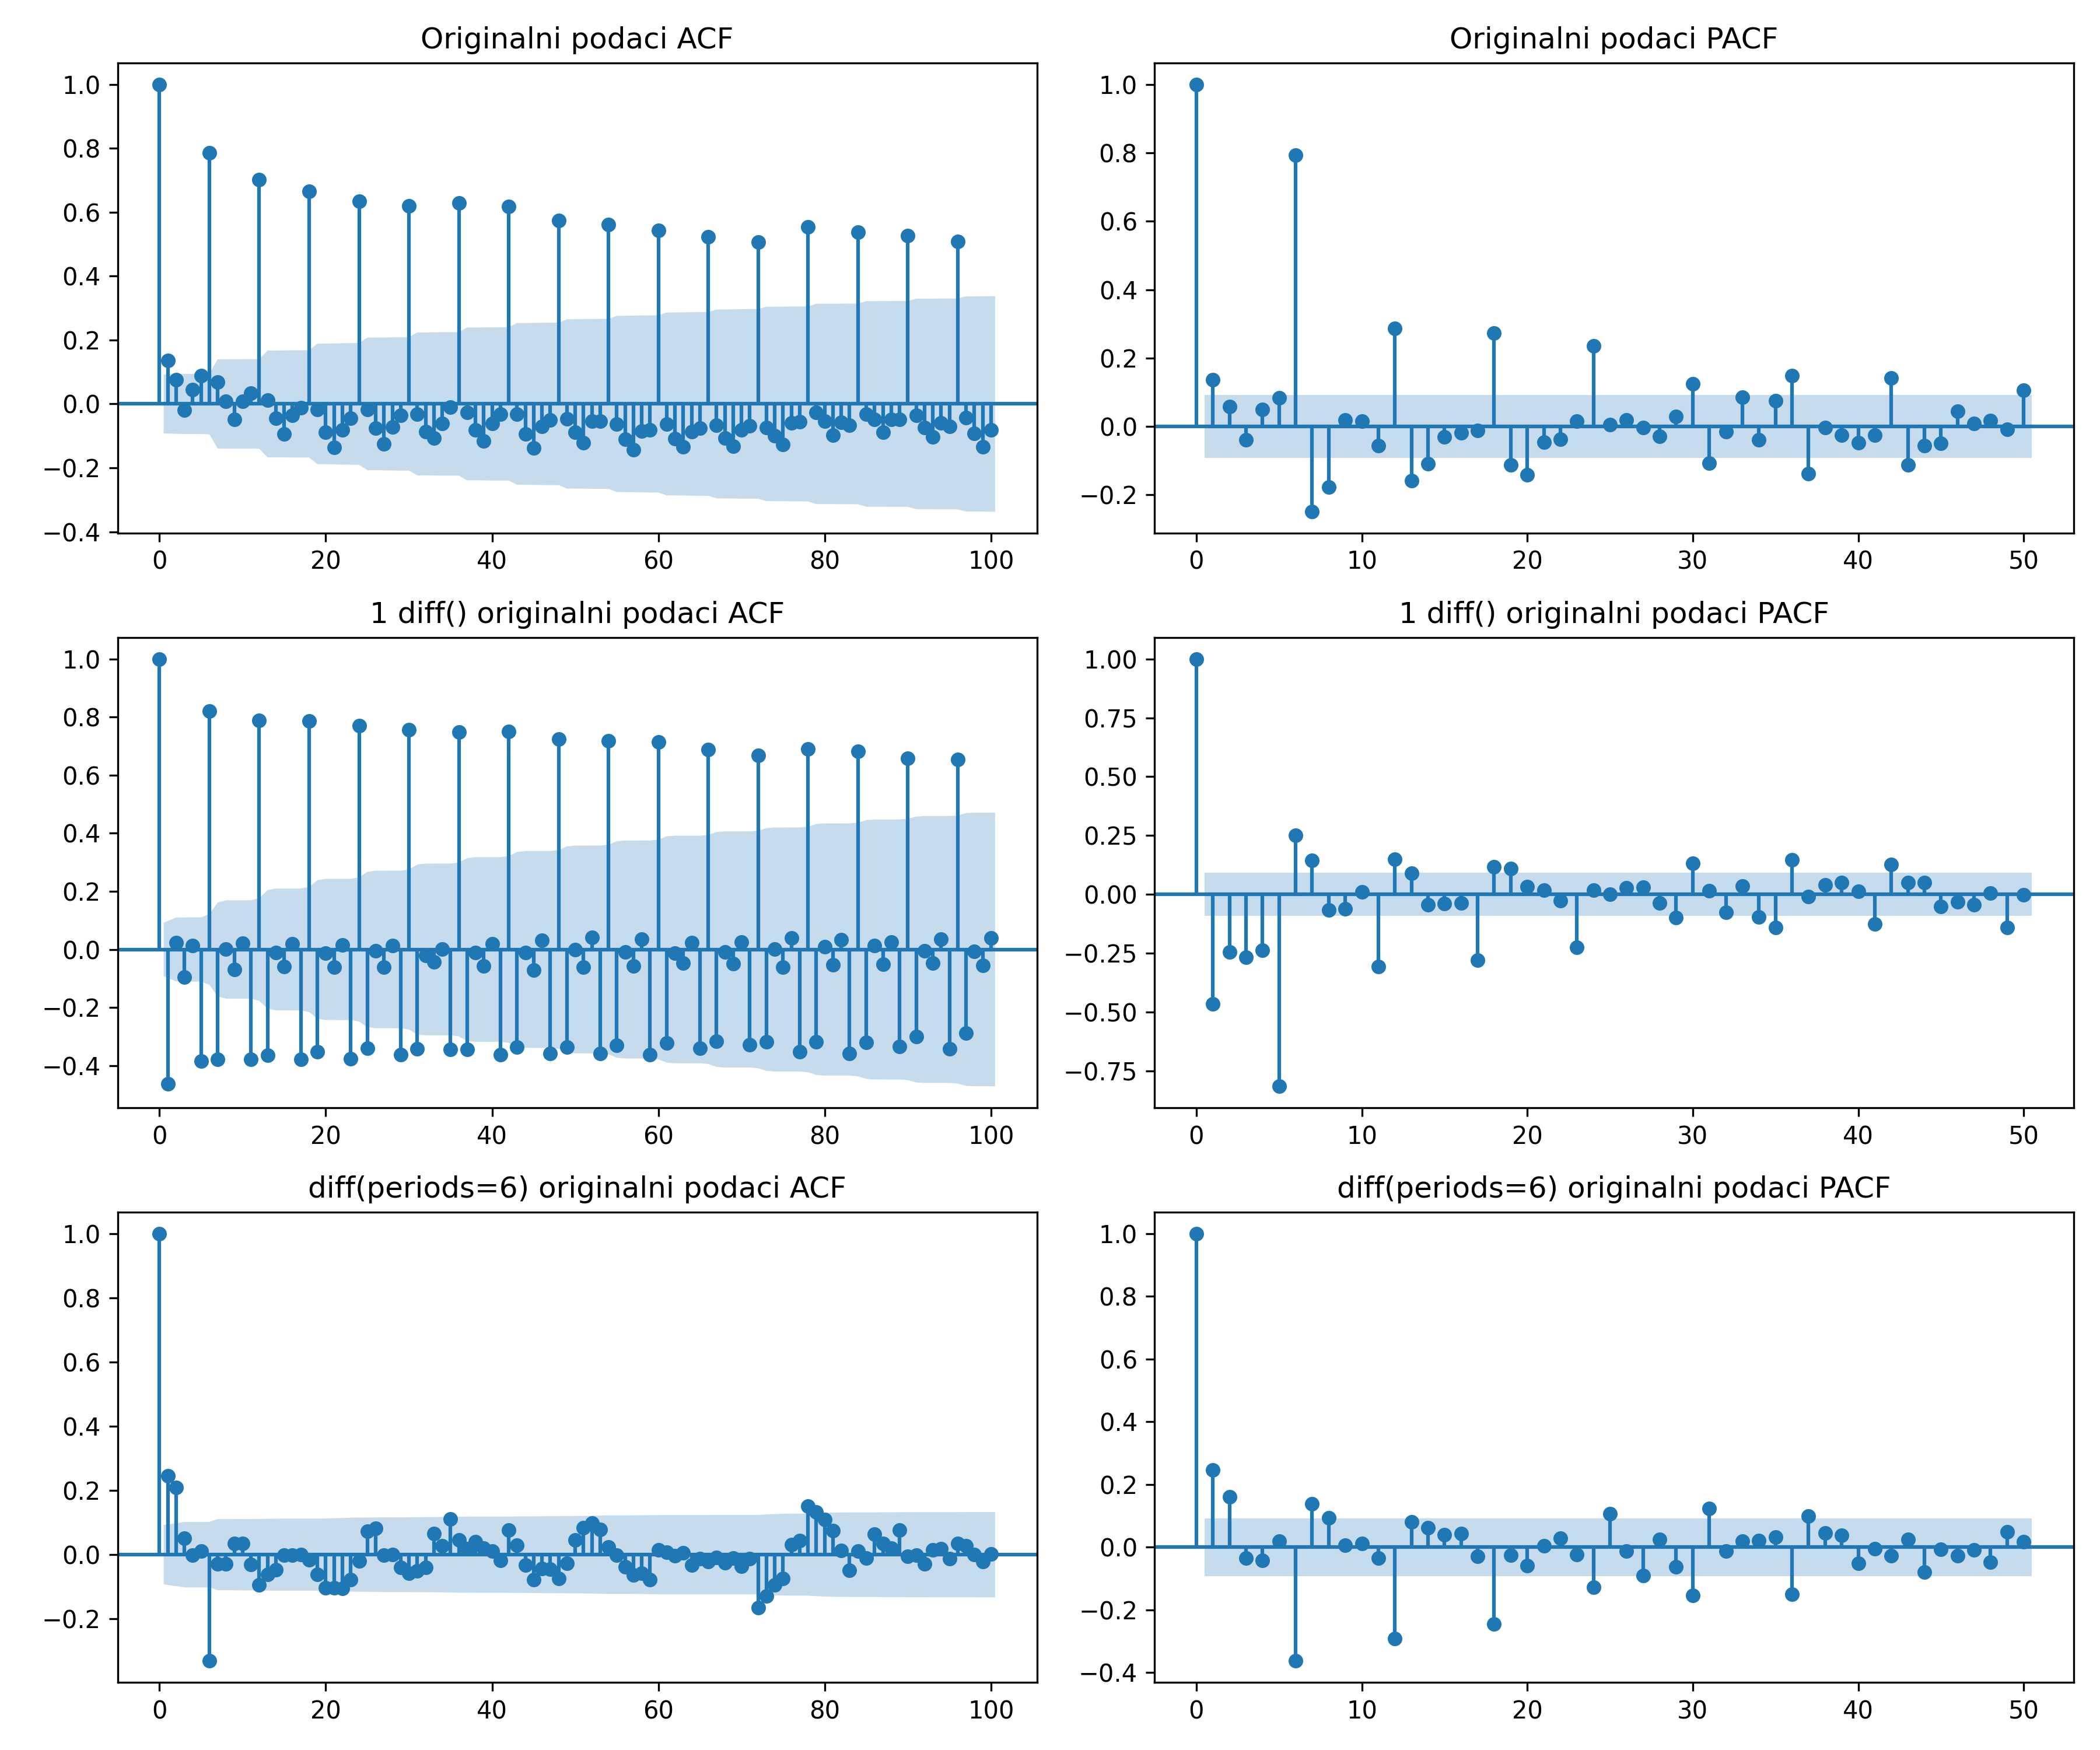
\includegraphics[width=1\textwidth]{./grafici/acf_pacf_dnevni.png}
  \caption{ACF i PACF grafici. Na x-osi su pomeraji, a na y-osi vrednost korelacije}
  \label{fig: acf_pacf_dnevni}
\end{figure}
Na osnovu ACF/PACF grafika, može se zaključiti da bi model ARIMA(0, 0, 0)(0, 0, 1)$_6$ mogao biti pogodan. U pitanju je sezonska ARIMA (SARIMA) koja ima vrednost MA=1, ali sa kašnjenjem od šest dana. Dakle, ovo sugeriše da za predviđanje ponedeljka treba gledati u vrednost greške predviđanja prethodnog ponedeljka, za predviđanje utorka vrednost greške predviđanja prethodnog utorka itd, jer je na vrednosti šest kod ACF grafika najviši špic, dok PACF grafik pokazuje opadanje vrednosti kroz sezonalne pomeraje. Isključivanjem nedelja iz podataka dnevne vremenske serije, dobijena je situacija da jedna sedmica ima šest dana, tako da dobijena vrednost od baš šest (a ne recimo sedam) u ovoj situaciji ima smisla. Ispitivanjem grafika raspodele reziduala (belog šuma), zaključeno je da u model treba uključiti i druge komponente, a ne samo sezonalnu MA komponentu.

\begin{table}[!ht]
\centering
\caption{SARIMA/ARIMA vrednosti AIC metrike}
\label{tbl: arime_aic}
\begin{tabular}{ |l|c| } 
\hline
MODEL & AIC \\
\hline
ARIMA(1, 0, 1) & 567.39\\ 
ARIMA(1, 0, 0) & 598.30\\ 
ARIMA(6, 0, 6) & 14.31\\ 
ARIMA(9, 0, 6) & 14.63\\
ARIMA(1, 0, 1)(1, 0, [1,2])$_6$ & 3.81\\
ARIMA(2, 0, 0)(2, 0, 1)$_6$ & 8.57\\
\hline
\end{tabular}
\end{table}

Pokretanjem automatskog procesa za određivanje najboljeg ARIMA modela, dobijen je model ARIMA(2, 0, 0)(2, 0, 1)$_6$. Kako su dva SARIMA modela sugerisala da treba gledati u jednu ili dve vrednosti šest dana u prošlost, ispitan je i model ARIMA(6, 0, 6) i model ARIMA(9, 0, 6) koji je isto dobijen automatskim procesom. Pored njih su iz radoznalosti ispitani i još neki modeli. Vrednosti AIC metrike ispitanih modela su prikazane u tabeli \ref{tbl: arime_aic}, vrednosti metrika evaluacije u tabeli \ref{tbl: arime_metrike}, a autokorelacioni grafik reziduala najboljeg modela na slici \ref{fig: reziduali}. Reziduali ne smeju da imaju korelaciju, tj. moraju predstavljati samo beli šum.

\begin{table}[!ht]
\centering
\caption{SARIMA/ARIMA metrike evaluacije}
\label{tbl: arime_metrike}
\begin{tabular}{ |l|c|c|c|c|} 
\hline
MODEL & MAE & MSE & RMSE & SMAPE \\
\hline
ARIMA(1, 0, 1) & 0.390 & 0.230 & 0.480 & 0.379 \\ 
ARIMA(1, 0, 0) & 0.383 & 0.216 & 0.465 & 0.376\\ 
ARIMA(6, 0, 6) & 0.564 & 0.094 & 0.307 & 0.213\\ 
ARIMA(9, 0, 6) & 0.209 & 0.095 & 0.309 & 0.224\\ 
ARIMA(1, 0, 1)(1, 0, [1,2])$_6$ & 0.192 & 0.095 & 0.308 & 0.208\\
ARIMA(2, 0, 0)(2, 0, 1)$_6$ & 0.200 & 0.092 & 0.304 & 0.216\\
\hline
\end{tabular}
\end{table}

\begin{figure}[!ht]
  \centering
  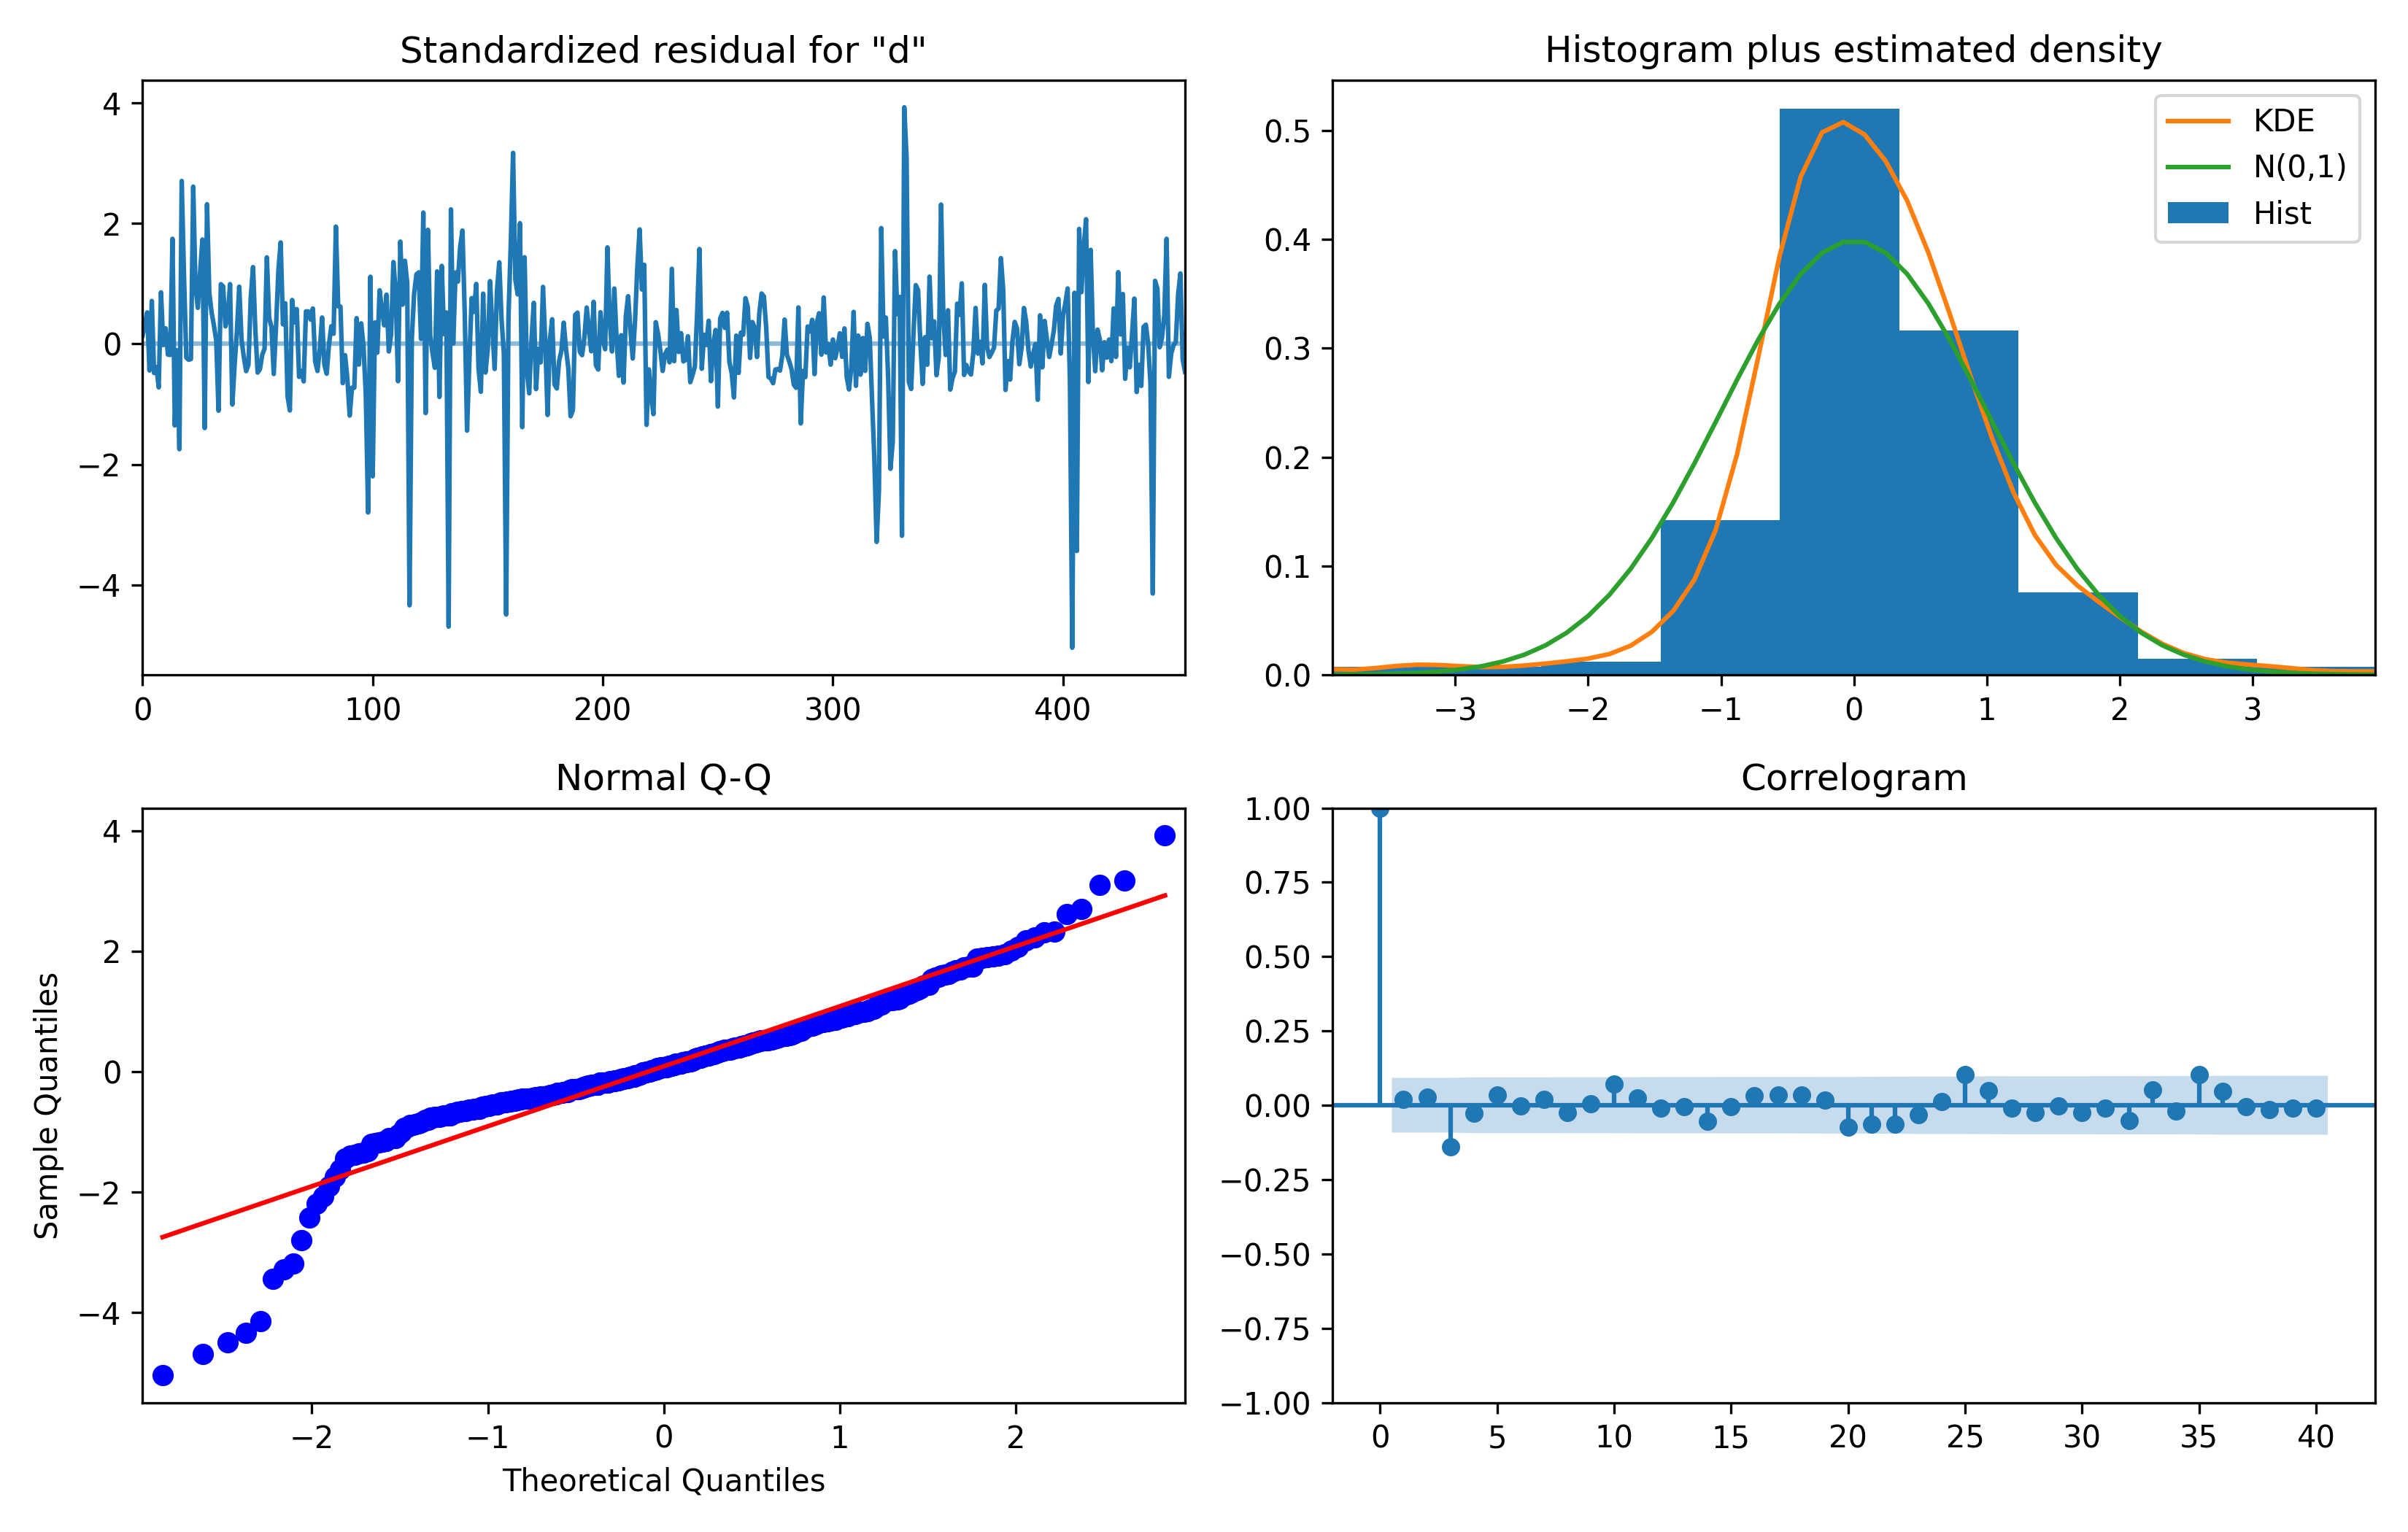
\includegraphics[width=1\textwidth]{./grafici/reziduali_arima.png}
  \caption{Provera normalnosti i odsustva korelacije među rezidualima modela ARIMA(1, 0, 1)(1, 0, [1, 2])$_6$}
  \label{fig: reziduali}
\end{figure}
Princip obučavanja pomenutih modela bio je da se u trening skupu na početku nalaze svi dani pre 01.03.2021. godine, a da se zatim predviđa jedan po jedan dan u budućnost, nakon čega se u trening skup dodaje jedan dan. Modeli su evaluirani na osnovu predviđanja jednog dana unapred od 01.03.2021. godine, treniranjem nad svim podacima pre. Takođe, predviđanja su vršena i odjednom po nekoliko dana unapred (konkretno 28 dana), da se ispita ponašanje modela. Na grafiku \ref{fig: test_arima} se može videti ponašanje dva modela.
\begin{figure}[!ht]
  \centering
  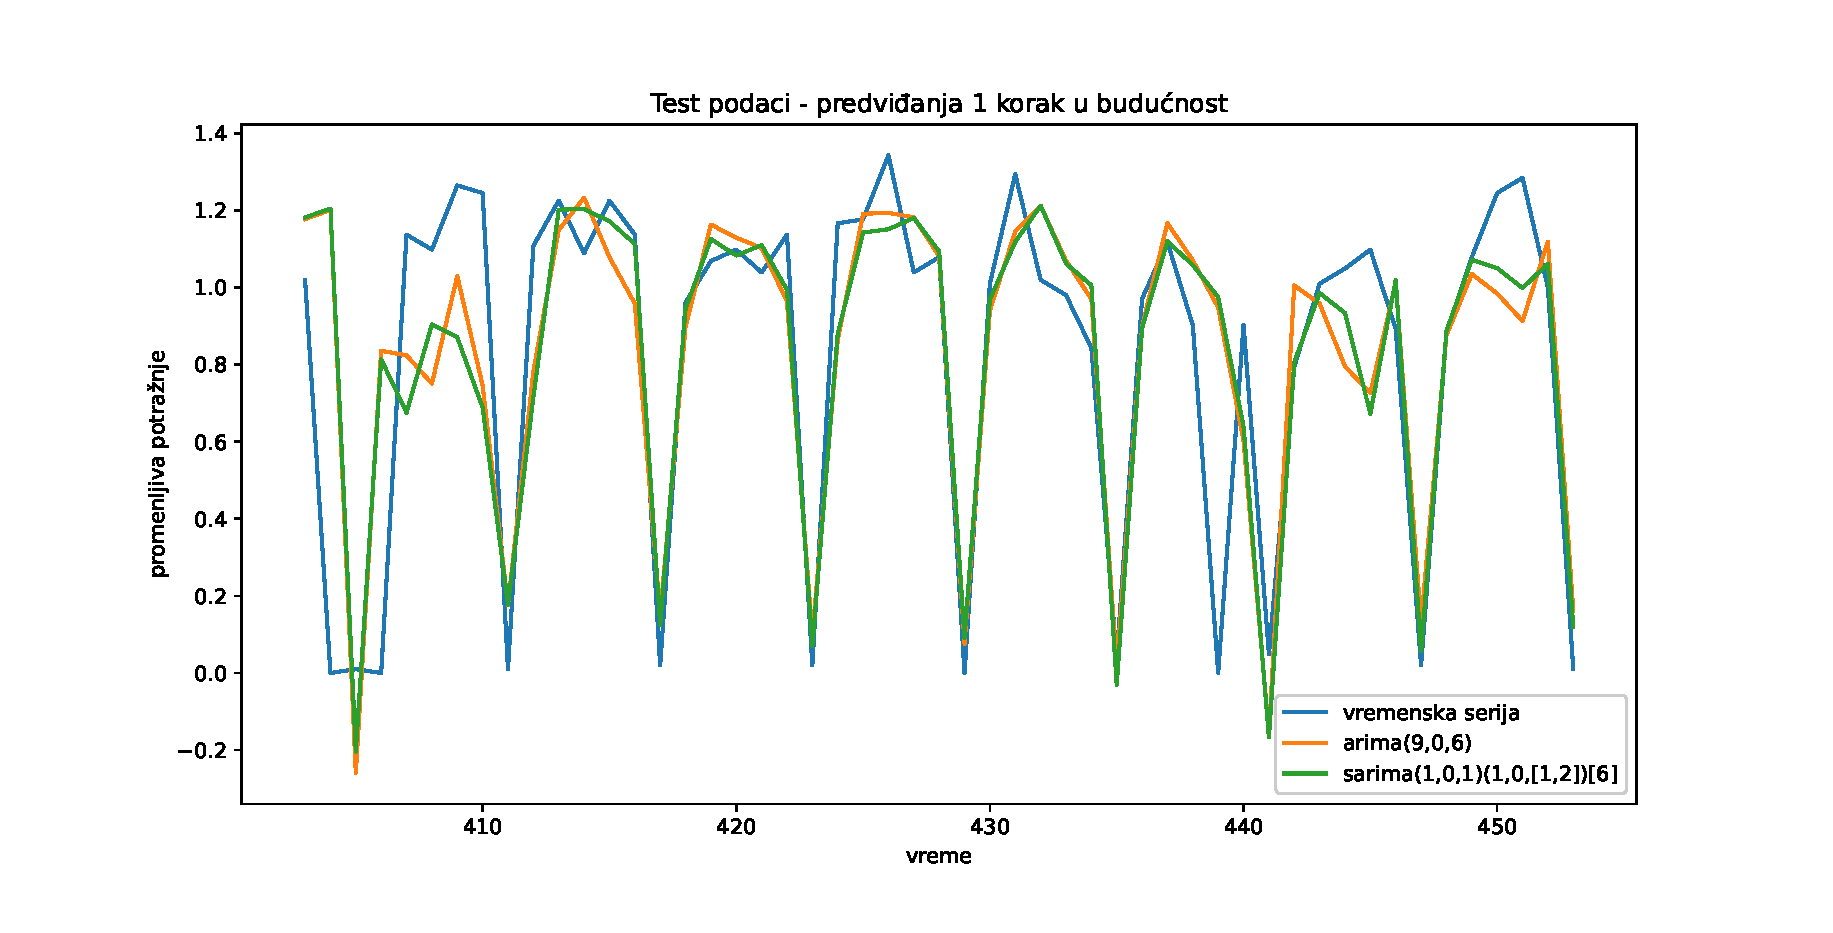
\includegraphics[width=1\textwidth]{./grafici/test_dnevna_arima.eps}
  \caption{Ponašanje jedan po jedan korak predviđanja dva modela kod ARIMA metode}
  \label{fig: test_arima}
\end{figure}

\subsection{Prophet}
Nad istim podacima i na isti način, isproban je i alat Prophet. Primenjena su četiri modela sa uključenim praznicima u Švedskoj, pošto je to omogućena opcija kod ovog metoda. Metrike evaluacije modela su prikazane u tabeli \ref{tbl: prophet_dnevni}, a grafik predviđanja na slici \ref{fig: test_prophet}. Sa grafika se može videti kako postoji jedan značajniji pad. Razlog tome je uračunavanje efekta praznika u modele, što je potvrdilo ideju da potencijalno treba uzimati u obzir praznike i u drugim modelima -- ukoliko je to moguće.
\begin{table}
\centering
\caption{Prophet metrike evaluacije}
\label{tbl: prophet_dnevni}
\begin{tabular}{ |l|c|c|c|c|} 
\hline
MODEL & MAE & MSE & RMSE & SMAPE \\
\hline
prophet (w, m, h) & 0.121 & 0.038 & 0.196 & 0.141 \\ 
prophet (w, m, h, flexible) & 0.113 & 0.032 & 0.180 & 0.130\\
prophet (d, w, m, h) & 0.119 & 0.035 & 0.188 & 0.139 \\
prophet (d, w, m, h, flexible) & 0.114 & 0.032 & 0.180 & 0.130\\
\hline
\end{tabular}
\end{table}

\begin{figure}[!ht]
  \centering
  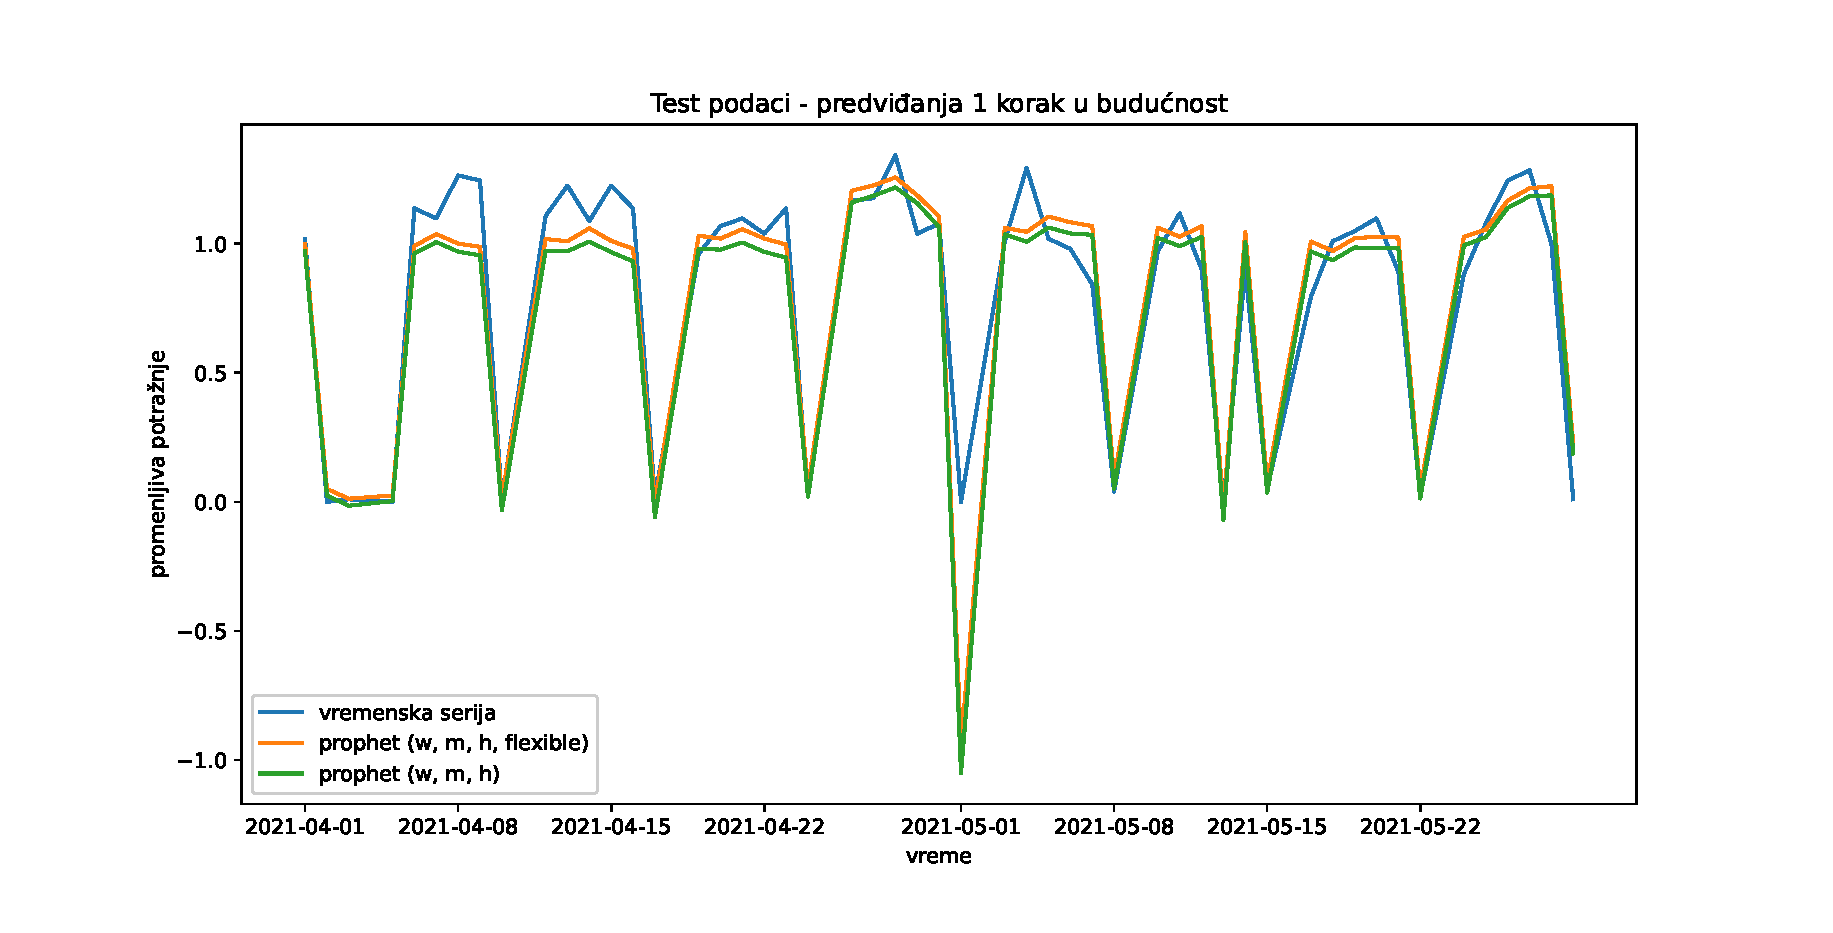
\includegraphics[width=1\textwidth]{./grafici/test_dnevni_prophet.eps}
  \caption{Ponašanje jedan po jedan korak predviđanja dva modela kod Prophet metode (test podaci počinju 01.04, jer je testirano predviđanje do 28 dana unapred od 01.03. i spajanjem skupova su izbačene nedostajuće vrednosti)}
  \label{fig: test_prophet}
\end{figure}
U tabeli su oznake koje predstavljaju informaciju da li su u model uključeni sezonalnost i praznici. Oznake su: w - uključena nedeljna sezonalnost, m - uključena mesečna sezonalnost, h - uključeni praznici, d - uključena dnevna sezonalnost i flexible - postavljanje parametra za definisanje trenda u modelu da bude fleksibilniji\footnote{\url{https://facebook.github.io/prophet/docs/trend_changepoints.html}}. 

\subsection{XGBoost}
XGBoost je isproban nad istim podacima, ali je sa njim urađen jedan eksperiment. Atributi za XGBoost nad dnevnim podacima su zapravo vrednosti promenljive potražnje (demand\_value) iz prethodnih nekoliko dana u prošlosti. Testirano je kako XGBoost radi sa trideset vrednosti iz prošlosti, sa tri dodata atributa koja predstavljaju praznike u Švedskoj.
Validacioni skup za XGBoost je predstavljao nasumičnih $20\%$ podataka dobijenih deljenjem celog trening skupa (koji predstavlja podatke pre vremenskog trenutka 01.03.2021. godine), za svrhe smanjenja preprilagođavanja tokom treniranja pomoću argumenta ranijeg stajanja. Metrike evaluacije za ovako dobijeni model su predstavljene u tabeli \ref{tbl: xgboost_1}. 
\begin{table}
\centering
\caption{XGBoost metrike evaluacije}
\label{tbl: xgboost_1}
\begin{tabular}{ |l|c|c|c|c|} 
\hline
MAE & MSE & RMSE & SMAPE \\
\hline
0.113 & 0.034 & 0.184 & 0.127 \\ 
\hline
\end{tabular}
\end{table}
Važnost atributa (\textit{eng.} feature importance) ovakvog modela je predstavljena na slici \ref{fig: vaznost_atributa}, sa koje se može zaključiti da XGBoost najveće težine (značaj) daje atributima koji predstavljaju vrednosti ciljne promenljive pre 6 dana, pre 18 dana i vrednosti da li je bio ili nije bio praznik tekućeg dana.
\begin{figure}[!ht]
  \centering
  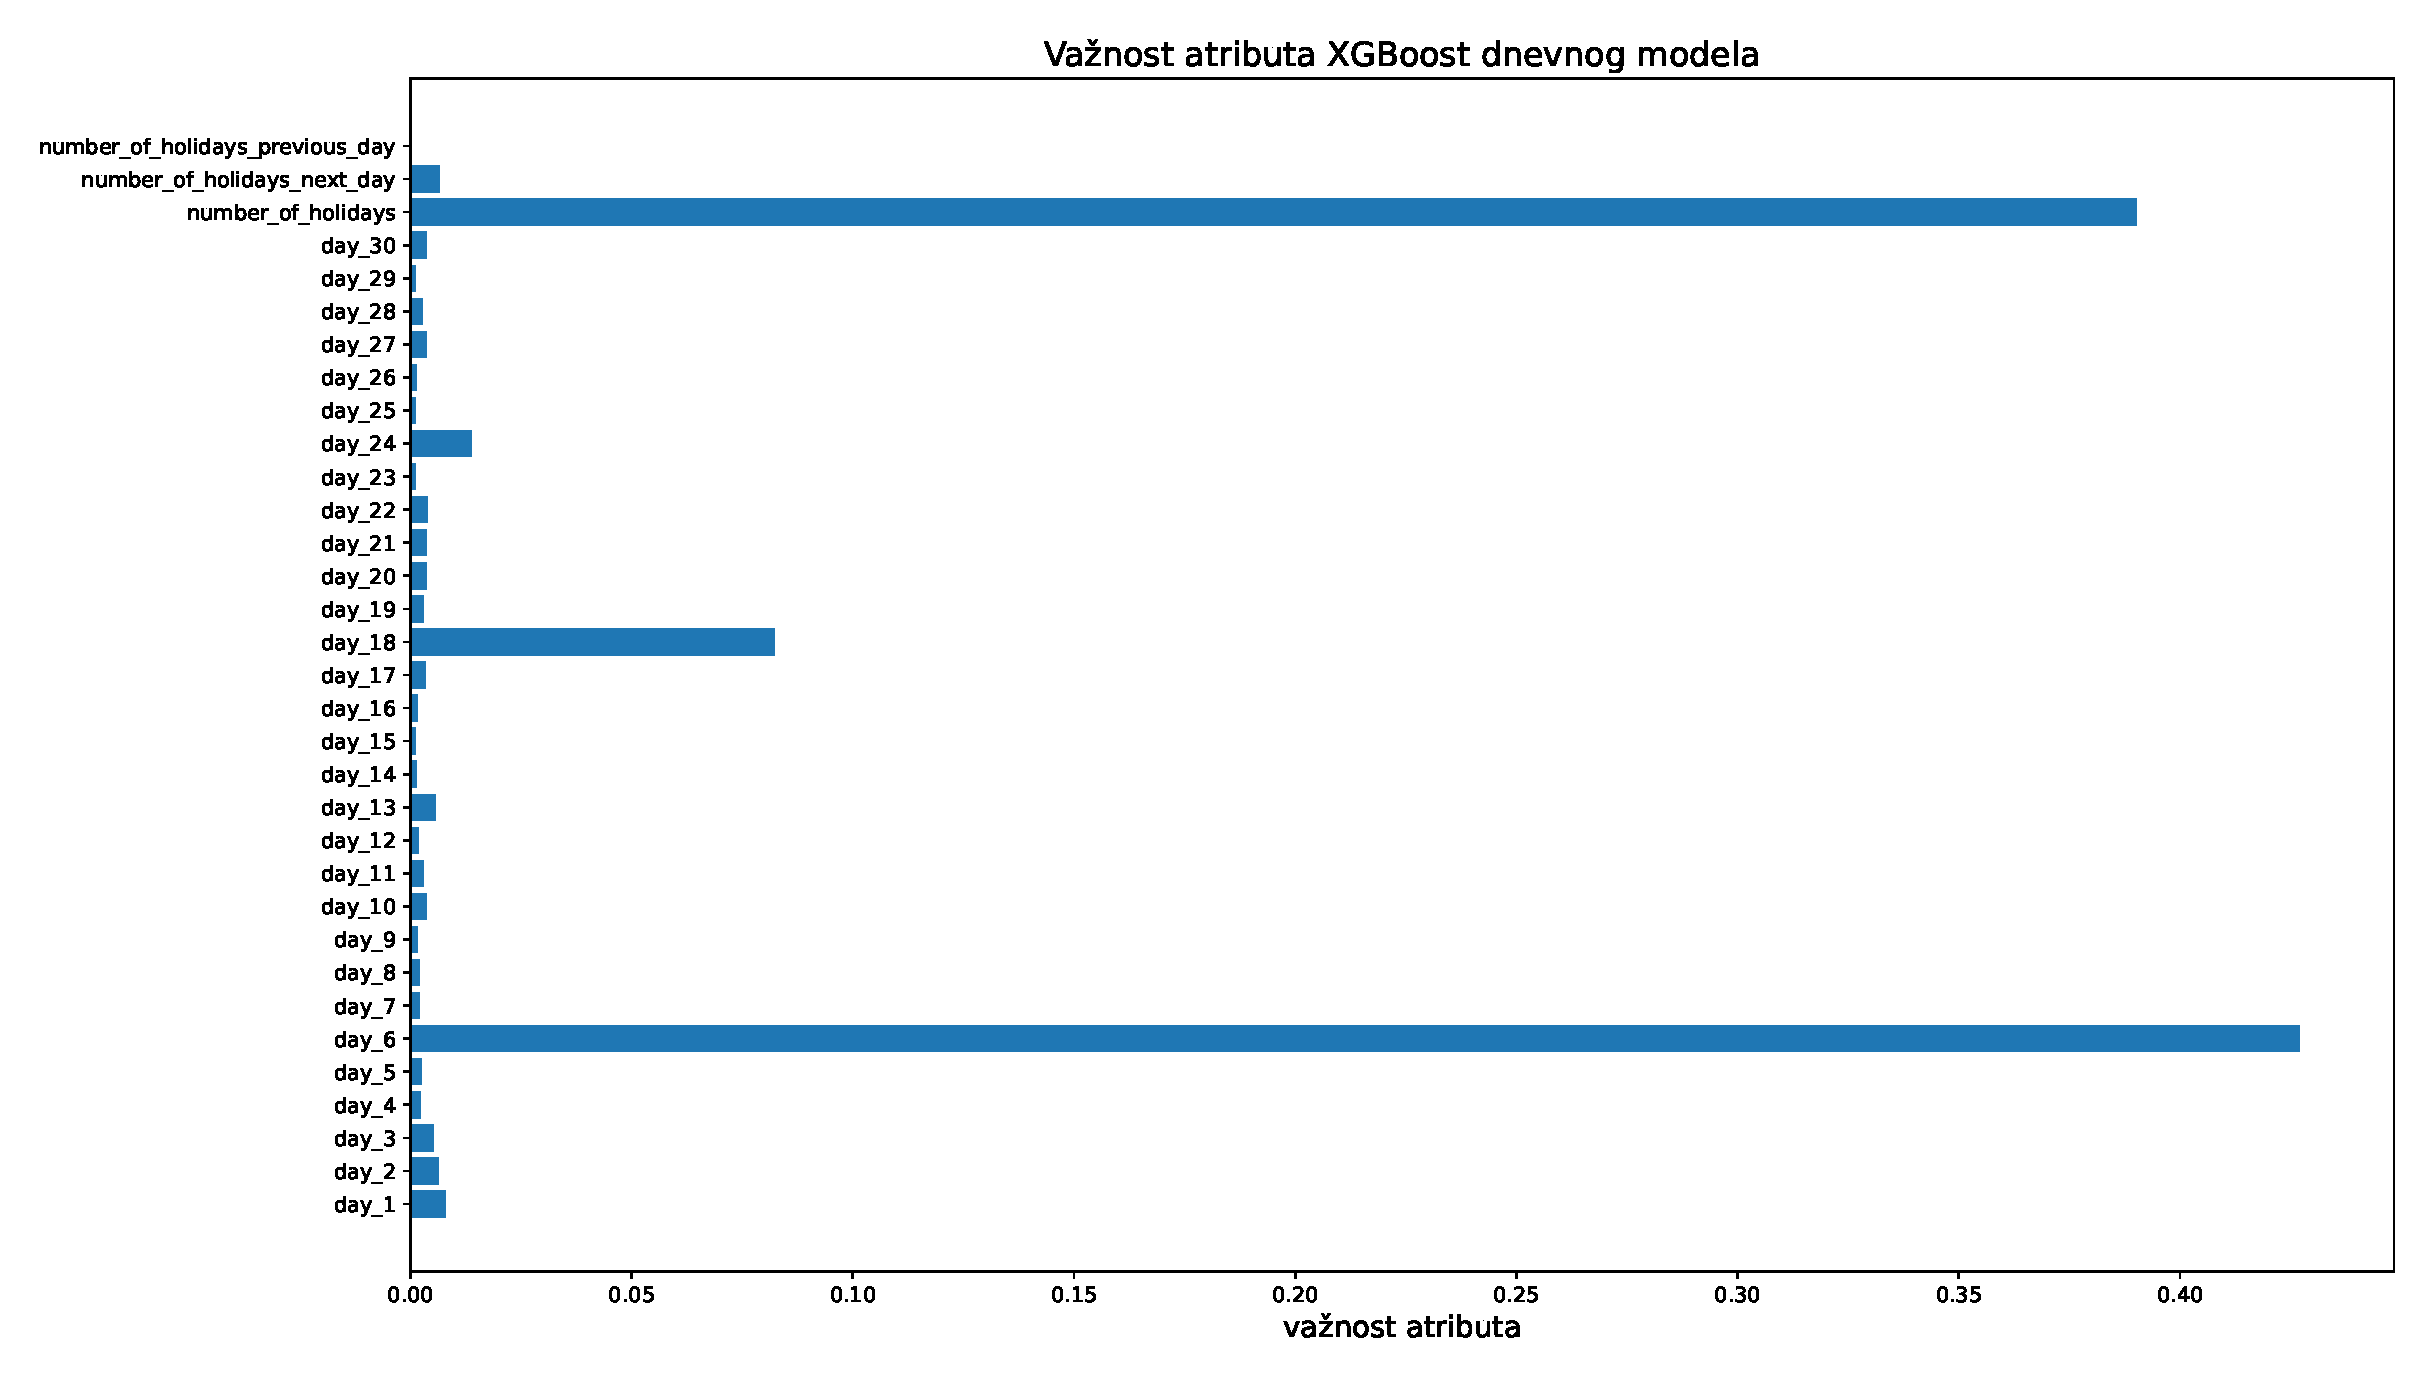
\includegraphics[width=1\textwidth]{./grafici/vaznost_atributa.eps}
  \caption{Važnost atributa kod XGBoost dnevnog modela}
  \label{fig: vaznost_atributa}
\end{figure}
Pored ovog, urađena su još dva eksperimenta. Prvi je bio dodavanje na postojeće atribute još jednog atributa, koji predstavlja prosek vrednosti prethodnih 6 dana. Drugi eksperiment je na prvobitne atribute dodao prosek razlike od srednje vrednosti za prethodnih 6 dana (pokušavajući da se imitira ARIMA model sa komponentom MA=6). Ovi eksperimenti su bili bezuspešni, sa atributima koji nisu doprineli poboljšanju modela. Na SHAP\footnote{SHapley Additive exPlanations je pristup koji može detaljnije da objasni izlaz bilo kog modela mašinskog učenja. Zasnovan je na Šapli vrednostima (\textit{eng.} Shapley values), konceptu koji dolazi iz teorije igara. Ove vrednosti kvantifikuju doprinos svakog igrača (ovde atributa) na igru (ovde na jedan posmatran izlaz).} grafiku \ref{fig: shap_beeswarm} se može pre svega primetiti kako manje vrednosti atributa koji predstavlja 6. dan iz prošlosti doprinosi smanjenju ciljne promenljive (i obrnuto), kao i kako veći broj praznika u danu doprinosi smanjenju vrednosti ciljne promenljive (i obrnuto). Svaka tačkica na slici \ref{fig: shap_beeswarm}, predstavlja jedan uzorak iz skupa. Na slici \ref{fig: shap_bar} predstavljena je apsolutna srednja vrednost SHAP vrednosti atributa. Ova analiza je urađena nad celim trening skupom osnovnog modela za koji su izložene metrike, kako bi se ispitalo ponašanje atributa, a prednost SHAP pristupa je što se po potrebi mogu ispitivati doprinosi atributa za svaki uzorak pojedinačno.

\begin{figure}[!htb]
    \centering
    \begin{subfigure}{.5\textwidth}
      \centering
      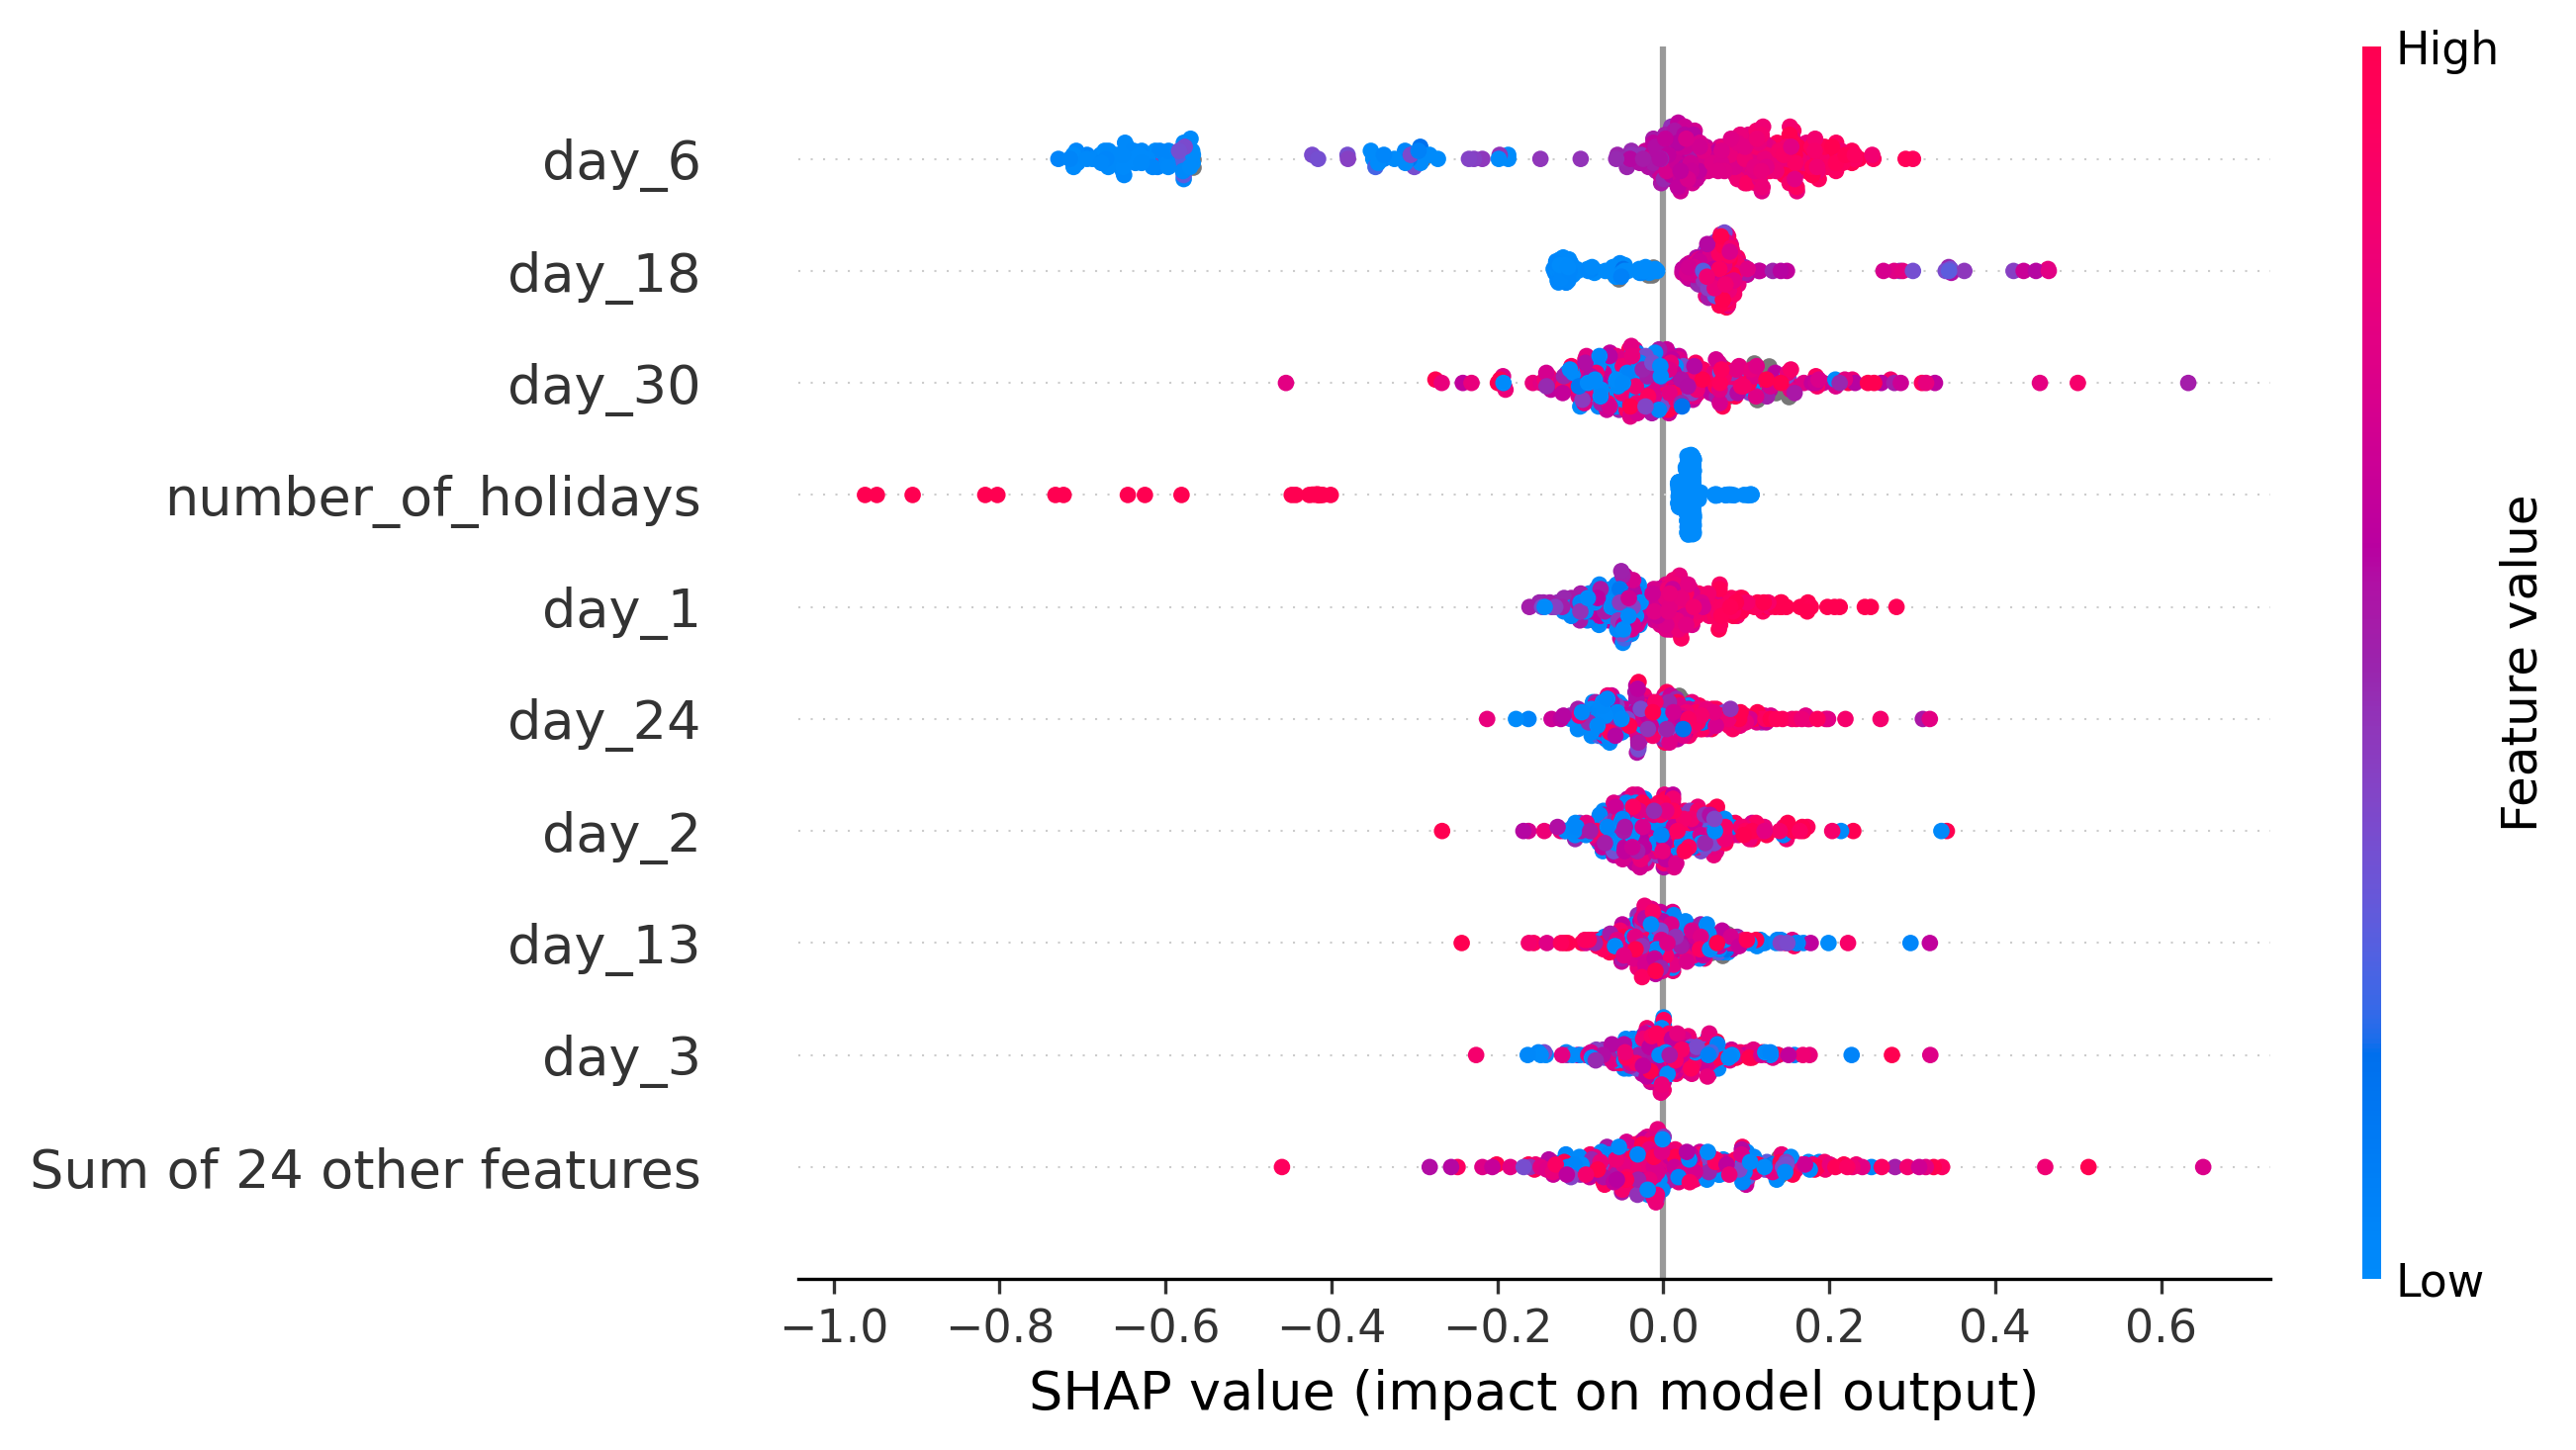
\includegraphics[width=1\linewidth]{./grafici/shap_xgboost_dnevni.png}
      \caption{Dijagram pčelinjak (\textit{eng.} beeswarm)}
      \label{fig: shap_beeswarm}
    \end{subfigure}%
    \begin{subfigure}{.5\textwidth}
      \centering
      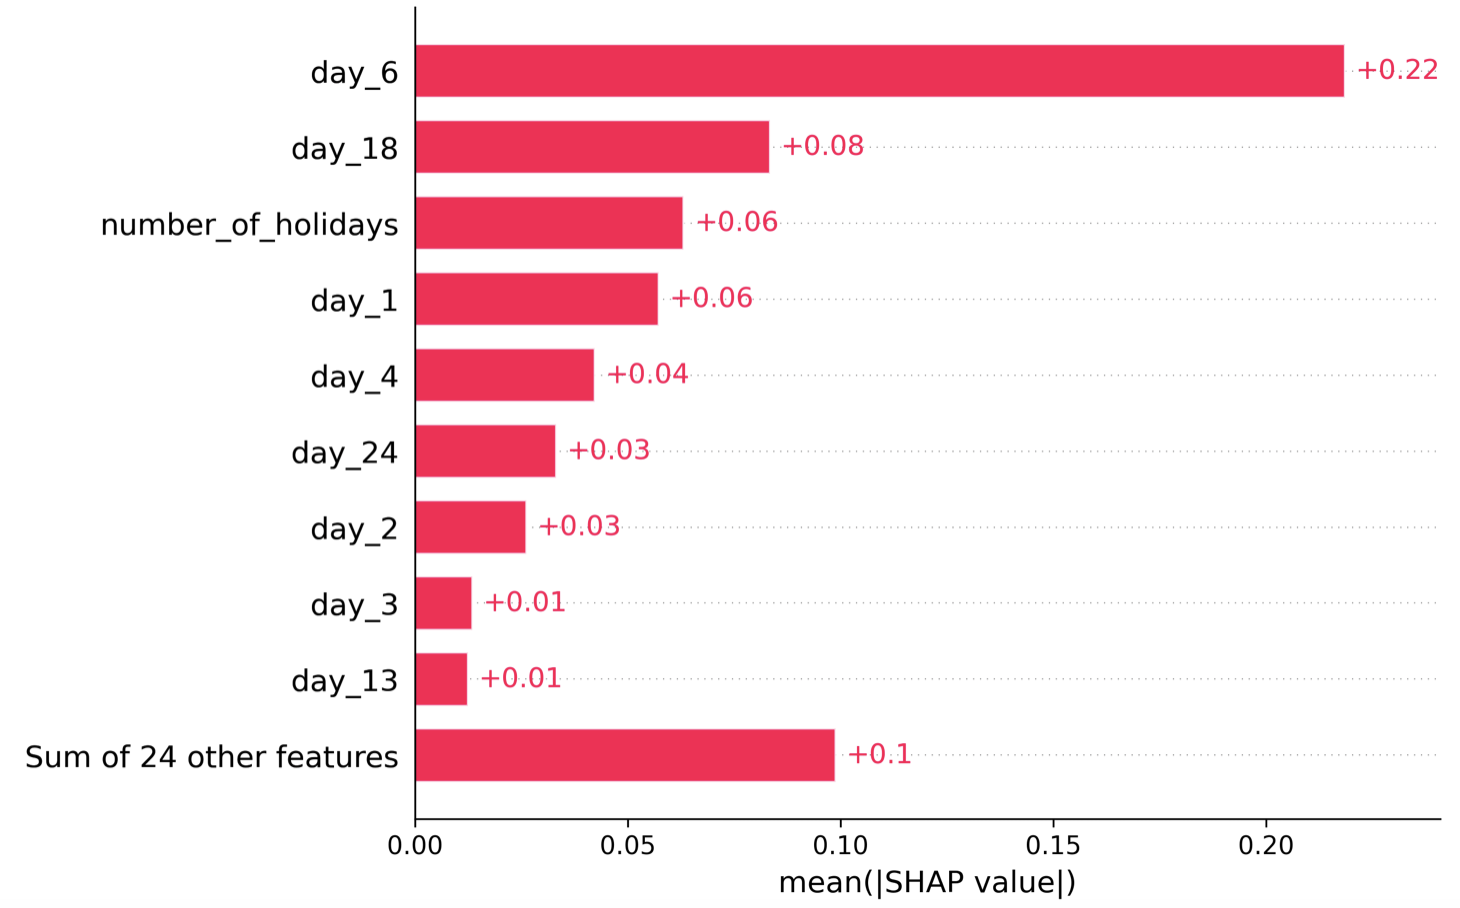
\includegraphics[width=1\linewidth]{./grafici/shap_xgboost_dnevni_bar.png}
      \caption{Stupičasti (\textit{eng.} bar) dijagram}
      \label{fig: shap_bar}
    \end{subfigure}
    \caption{SHAP vrednosti nad celim trening skupom}
    \label{fig: shap_xgboost}
\end{figure}

\section{Nedeljni nivo - na nivou države}
Primer podataka grupisanih na nedeljnom nivou, može se videti u tabeli \ref{tbl: weekly_data_example}. Ta vremenska serija je predstavljena na grafiku \ref{fig: nedeljna_serija}. Ukupan broj dostupnih nedelja je 76. Prvo što se može primetiti kod ove vremenske serije su dva veća pada vrednosti. Jedan se desio oko Uskrsa 2020. godine, a drugi se desio oko Nove godine.
\begin{figure}[!ht]
  \centering
  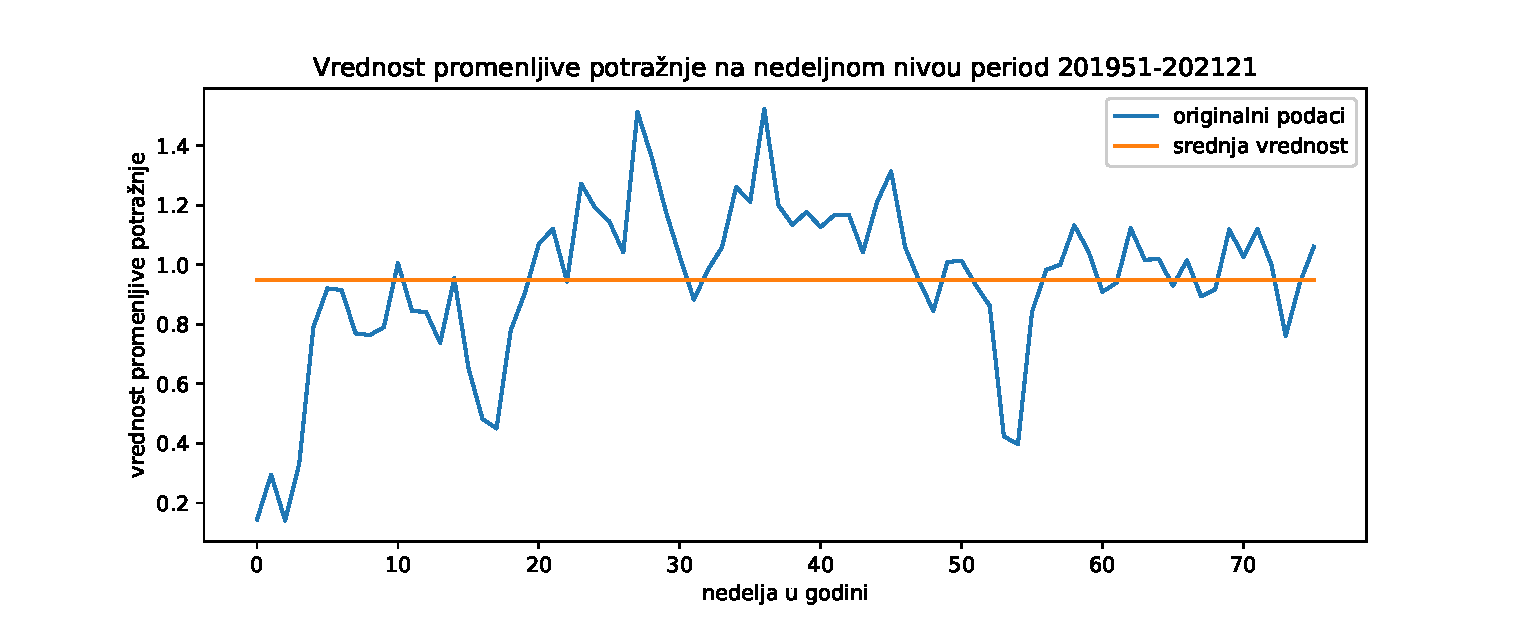
\includegraphics[width=1\textwidth]{./grafici/nedeljna_vremenska_serija.eps}
  \caption{Nedeljna vremenska serija}
  \label{fig: nedeljna_serija}
\end{figure}
\subsection{ARIMA i Prophet}
Kao i kod primera nad dnevnim podacima, prva ispitivana stvar je stacionarnost vremenske serije, za čiju proveru je korišćen statistički test stacionarnosti -- uvećan Diki-Fuler test. Vrednosti rezultata testa nad nedeljnim podacima su sledeći:
\begin{minipage}{\linewidth}
\vspace{15pt}
\begin{verbatim}
Test Statistics                -3.915460
p-value                         0.001924
No. of lags used                0.000000
Number of observations used    75.000000
critical value (1%)            -3.520713
critical value (5%)            -2.900925
critical value (10%)           -2.587781
\end{verbatim}
\vspace{10pt}
\end{minipage}
Može se zaključiti da je serija stacionarna i da bi vrednost parametra d trebala da bude nula, tj. da nema potrebe za diferenciranjem podataka. Kako se radi o nedeljnim podacima, za svaku nedelju (sedmicu) su sigurno dostupni neki podaci, tako da ne postoje nedostajuće nedelje. Na grafiku \ref{fig: acf_pacf_nedeljni} su prikazani grafici ACF i PACF, sa ciljem da se bolje razume ponašanje serije i da se odrede najpogodnije vrednosti parametara p i q. Sa grafika vremenske serije se može zaključiti da nema nekih lako uočljivih sezonalnosti, za dostupnu količinu podataka, a to potvrđuju i ACF/PACF plotovi. 
\begin{figure}[!ht]
  \centering
  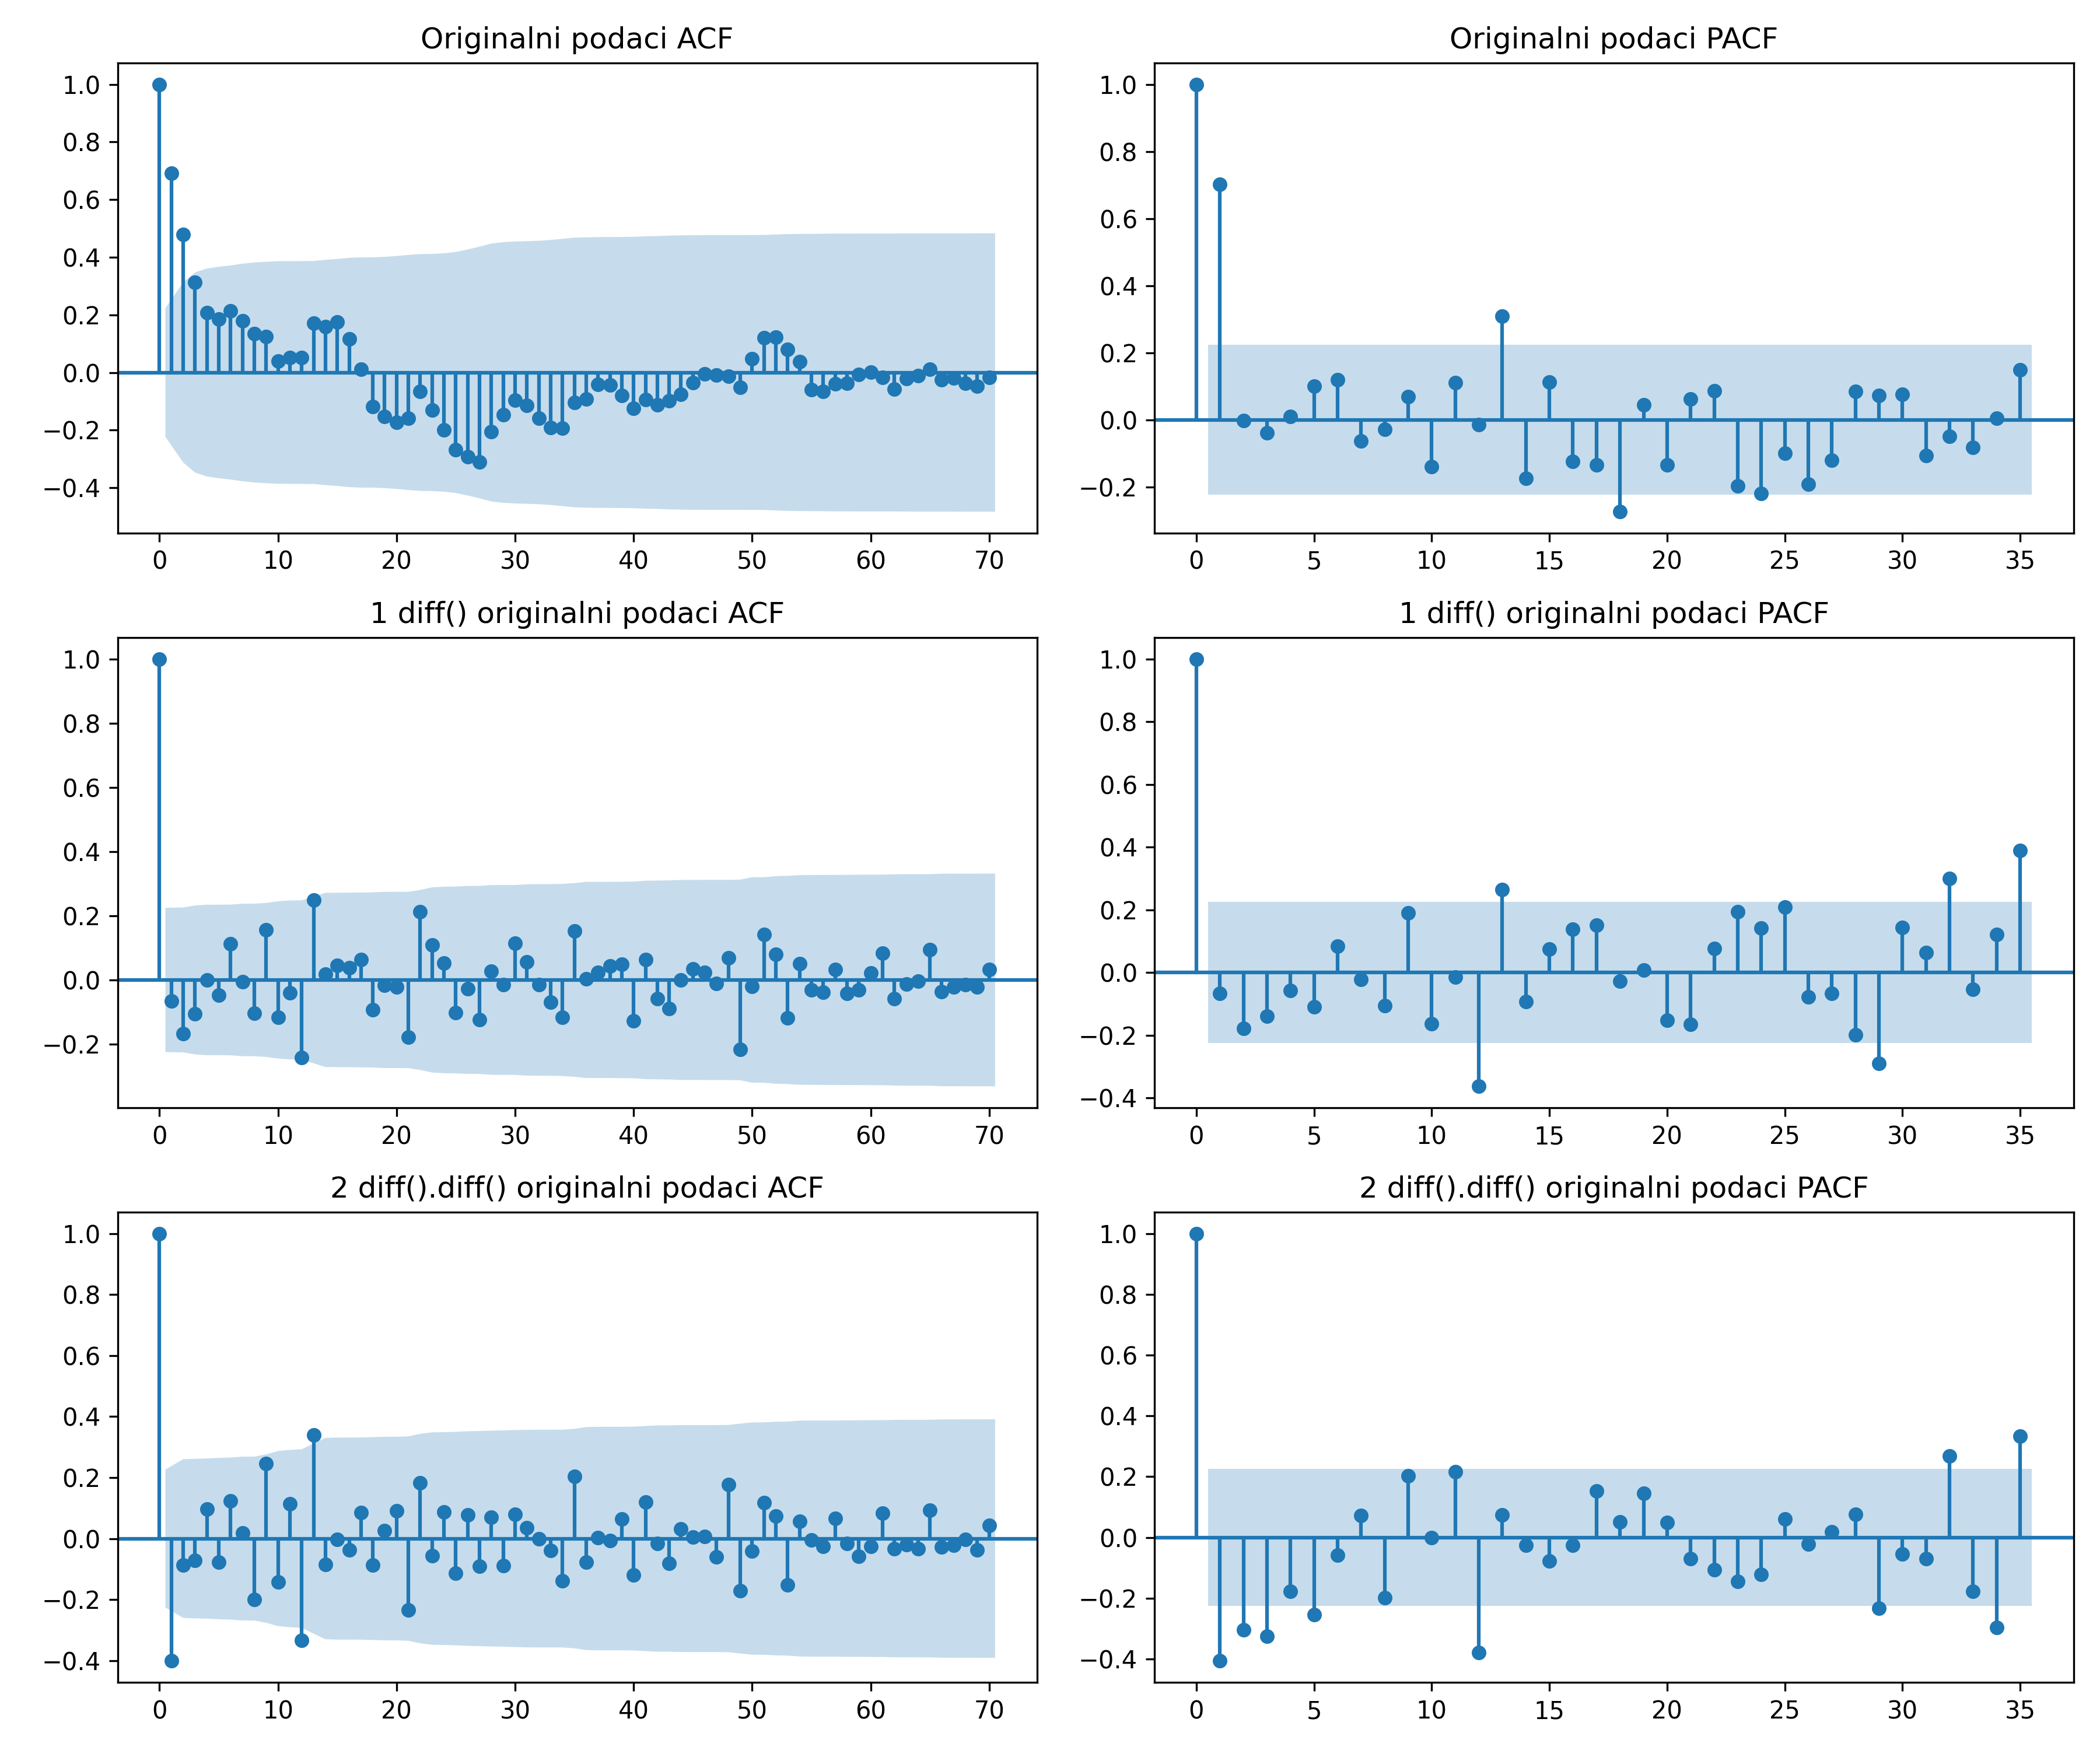
\includegraphics[width=1\textwidth]{./grafici/acf_pacf_nedeljni.png}
  \caption{ACF i PACF grafici (x-osi su kašnjenja, a na y-osi vrednosti korelacije)}
  \label{fig: acf_pacf_nedeljni}
\end{figure}
Ono što se praćenjem literature zaključilo je da pogodan model može da bude ARIMA(1, 0, 2). Postoji jedan špic izvan značajne zone na PACF grafiku, do prvog sledećeg špica unutar zone, što određuje AR parametar. Na ACF grafiku se primećuju dva špica izvan značajne zone, tako da je to jedan indikator da je parametar $MA=2$. Model koji je automatska funkcija koja sve ovo radi vratila kao najbolji prema AIC metrici je ARIMA(1, 0, 0), dakle čist autoregresivni model koji predviđanja pravi isključivo na jednoj prethodnoj vrednosti cilje promenljive. Pored ovih modela isprobani modeli su i: ARIMA(1, 1, 1), ARIMA(12, 1, 0) i ARIMA(13, 0, 2). Za model ARIMA(13, 0, 2) razlog je što PACF pokazuje značajan špic na vrednosti kašnjenja (laga) 13, a ostali su isprobani iz radoznalosti. Rezultati AIC metrika za ARIMA modele su prikazani u tabeli \ref{tbl: arima_aic_nedeljna}.
\begin{table}[!ht]
\centering
\caption{AIC metrika za ARIMA modele nad nedeljnim podacima}
\label{tbl: arima_aic_nedeljna}
\begin{tabular}{ |l|c|} 
\hline
MODEL & AIC \\
\hline
ARIMA(1, 0, 0) & -45.564\\
ARIMA(1, 1, 1) & -43.280\\
ARIMA(1, 0, 2) & -41.935\\
ARIMA(12, 1, 0) & -39.918\\
ARIMA(13, 0, 2) & -35.865\\
\hline
\end{tabular}
\end{table}
Iz tabele se može primetiti da postoji bolji model po AIC vrednosti od modela koji je automatska funkcija predložila. Nad test podacima su evaluirane metrike i ta statistika je prikazana u tabeli \ref{tbl: nedeljna_serija_metrike}. Pored ARIMA modela, isprobana su i dva Prophet modela, koja su se istraživanjem pokazala kao najbolja.
\begin{table}
\centering
\caption{Evaluacione metrike nad test podacima nedeljne vremenske serije}
\label{tbl: nedeljna_serija_metrike}
\begin{tabular}{ |l|c|c|c|c|} 
\hline
MODEL & MAE & MSE & RMSE & SMAPE\\
\hline
prophet (w, m, h) & 0.180 & 0.052 & 0.227 & 0.164\\
prophet (w, m, h, flexible) & 0.145 & 0.038 & 0.195 & 0.144\\
ARIMA(1, 0, 0) & 0.155 & 0.041 & 0.203 & 0.151\\
ARIMA(1, 1, 1) & 0.162 & 0.046 & 0.216 & 0.155\\
ARIMA(1, 0, 2) & 0.159 & 0.042 & 0.205 & 0.154\\
ARIMA(12, 1 ,0) & 0.163 & 0.046 & 0.215 & 0.157\\
ARIMA(13, 0, 2) & 0.162 & 0.044 & 0.210 & 0.158\\
\hline
\end{tabular}
\end{table}
Na grafiku \ref{fig: nedeljni_test} su predstavljene predikcije nad test podacima nekoliko modela.
\begin{figure}[!ht]
  \centering
  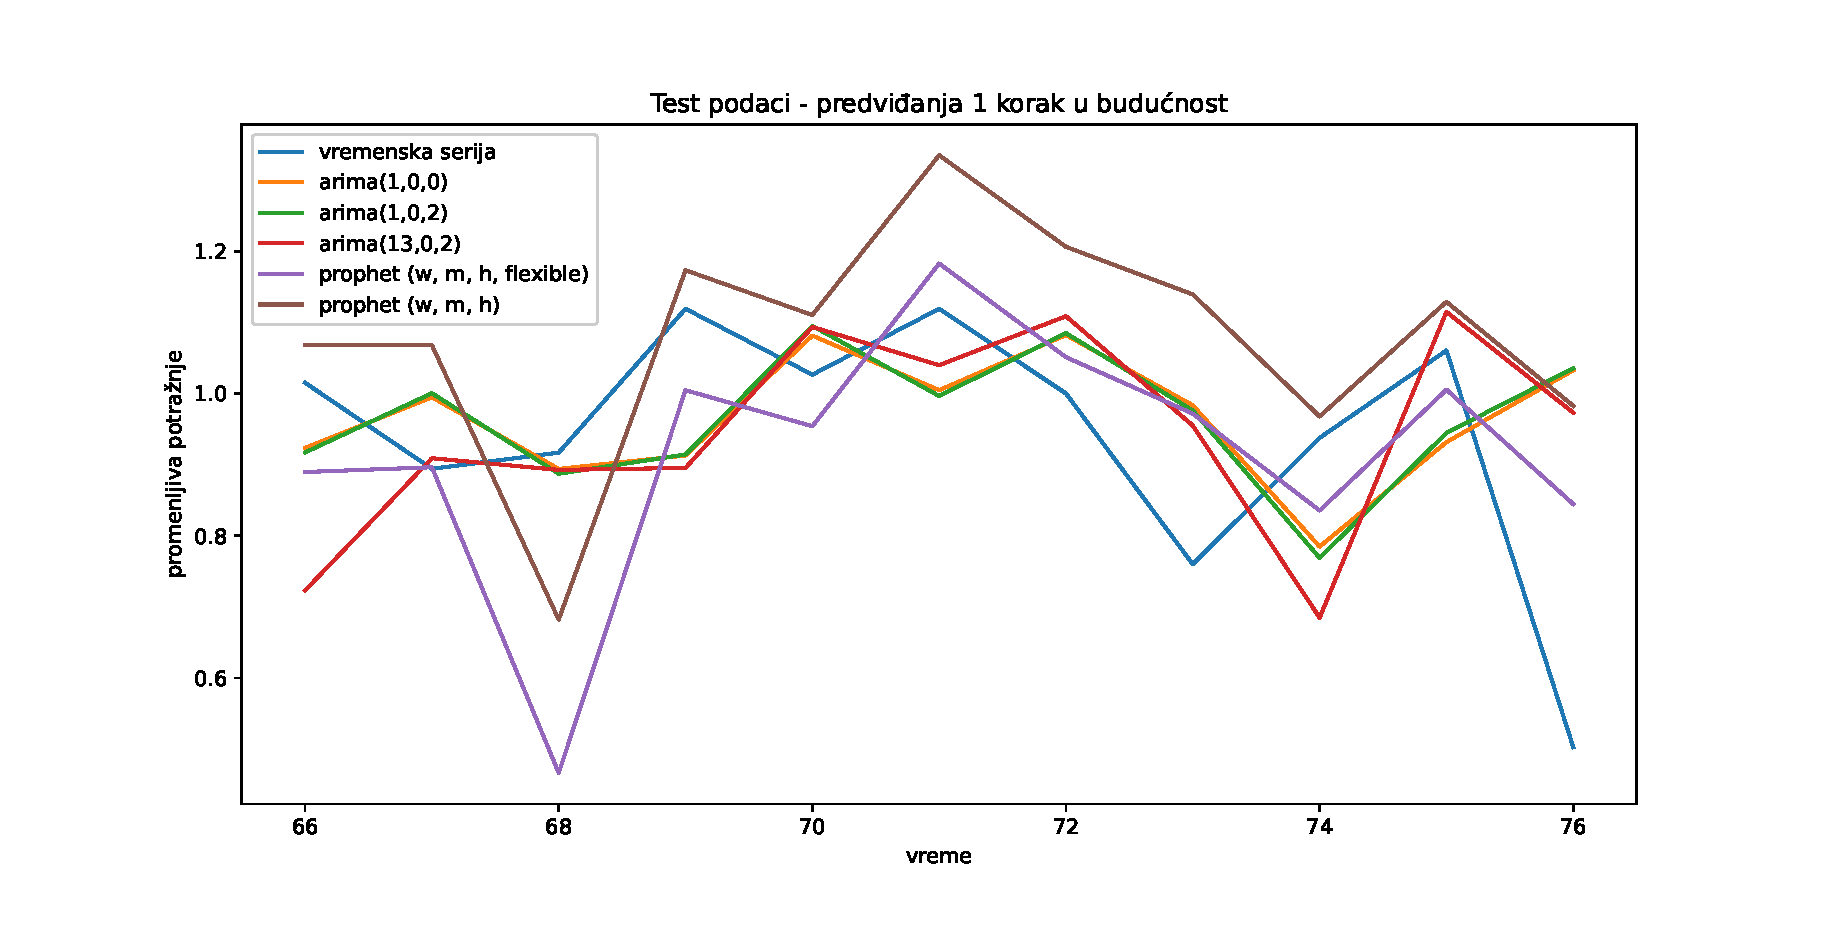
\includegraphics[width=1\textwidth]{./grafici/test_nedeljni_modeli.eps}
  \caption{Predviđanja nad test skupom za nekoliko modela nad nedeljnom vremenskom serijom}
  \label{fig: nedeljni_test}
\end{figure}

\subsection{XGBoost}
Kao i kod dnevnih podataka, slično je urađeno i nad nedeljnim podacima. Atributi za XGBoost nad nedeljnim podacima su vrednosti promenljive potražnje na nedeljnom nivou, iz prethodnih nekoliko nedelja (konkretno ovde devet nedelja). Dodata su i tri atributa koja predstavljaju praznike u Švedskoj, na isti način kao i za dnevne podatke, samo sumirani na nedeljnom nivou. Metrike evaluacije za ovako dobijeni model su predstavljene u tabeli \ref{tbl: xgboost_nedeljni_metrike}, a važnost atributa je predstavljena na grafiku \ref{fig: xgboost_nedeljno_importance}.

\begin{table}
\centering
\caption{Metrike evaluacije nad test podacima nedeljnog XGBoost modela}
\label{tbl: xgboost_nedeljni_metrike}
\begin{tabular}{ |l|c|c|c|} 
\hline
MAE & MSE & RMSE & SMAPE\\
\hline
0.146 & 0.046 & 0.215 & 0.139\\
\hline
\end{tabular}
\end{table}
\begin{figure}[!ht]
  \centering
  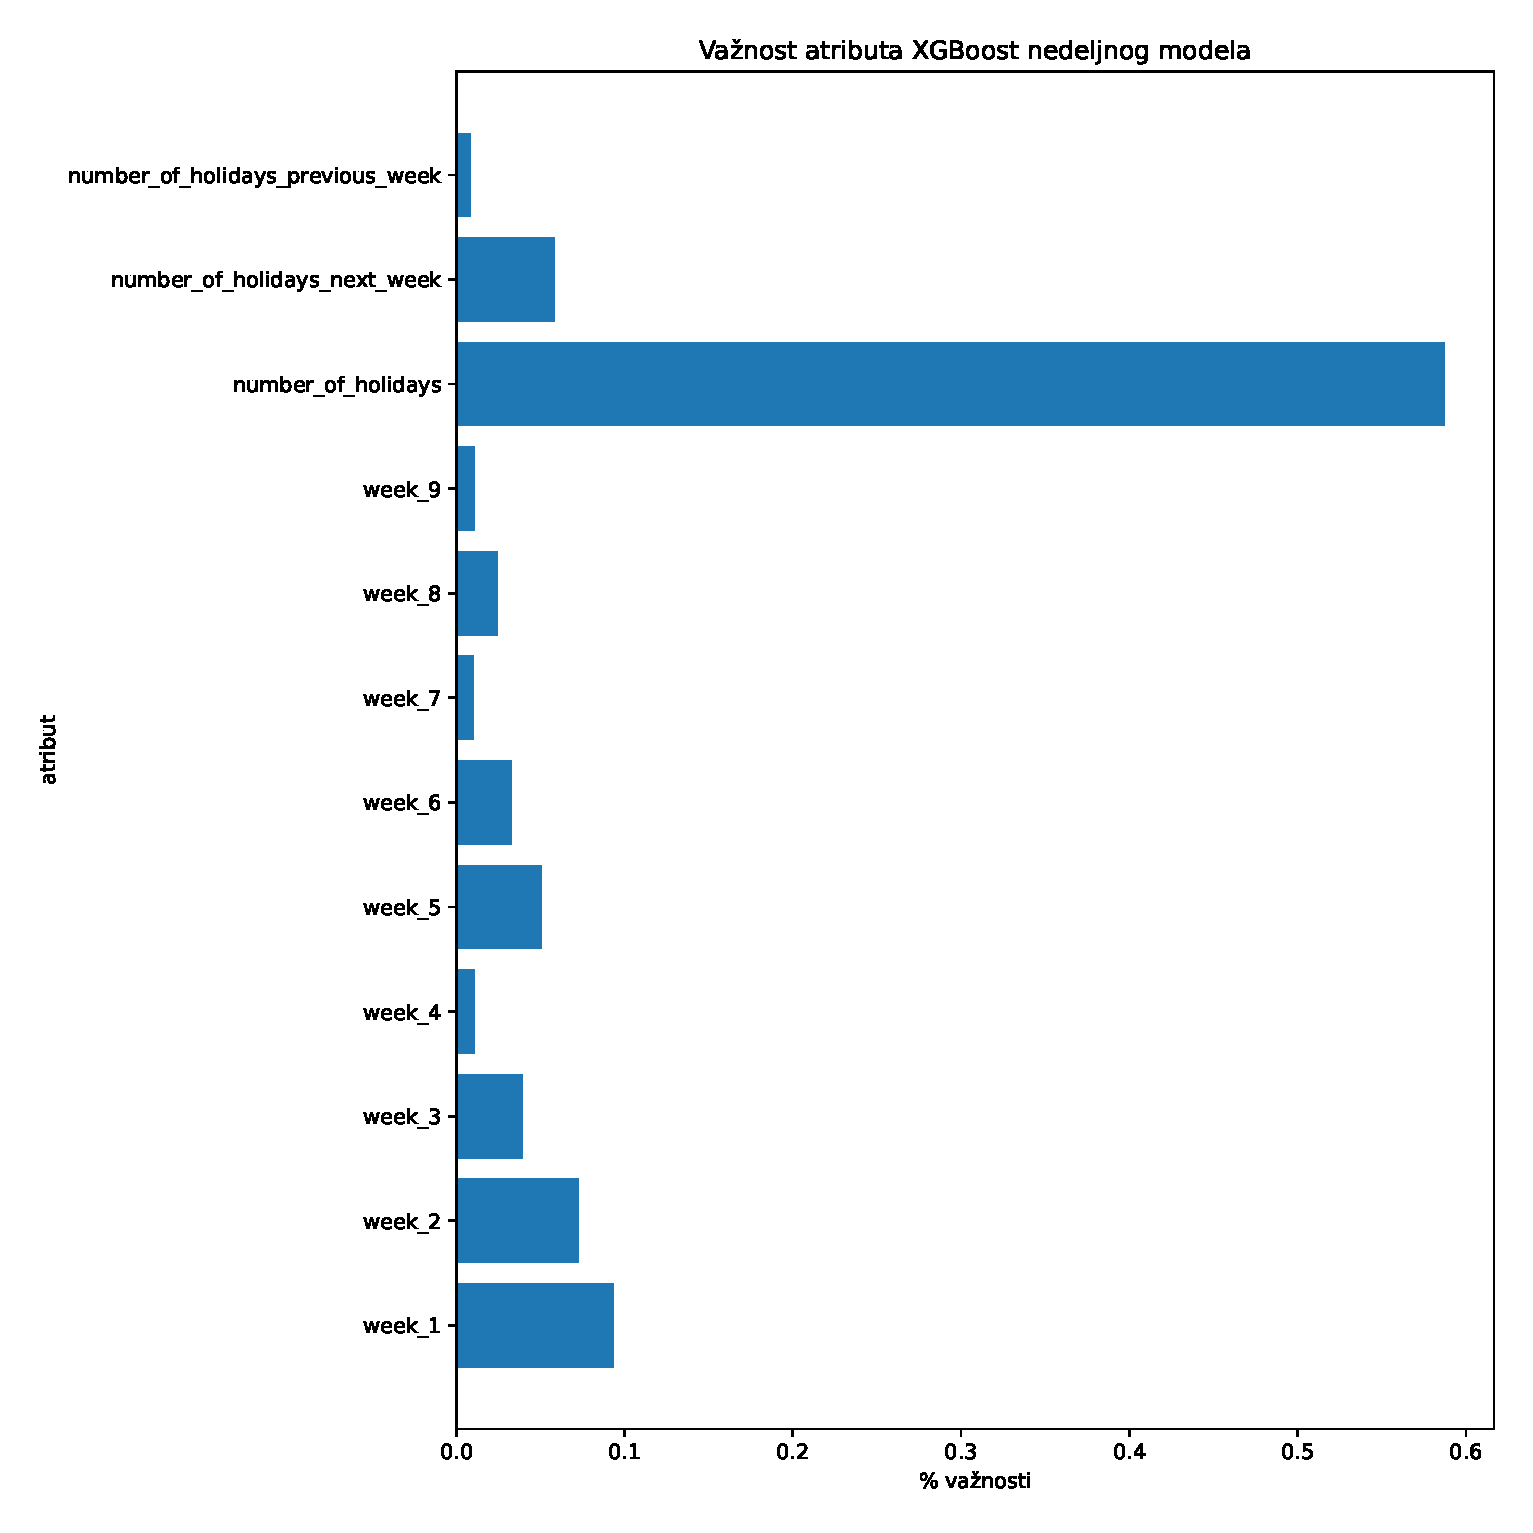
\includegraphics[width=0.7\textwidth]{./grafici/xgboost_nedeljni_vaznost_atributa.eps}
  \caption{Važnost atributa kod XGBoost nedeljnog modela}
  \label{fig: xgboost_nedeljno_importance}
\end{figure}

\section{XGBoost veća granularnost - na nivou automehaničarskih radnji i marki automobila}
Kako se dosadašnji tok rada bavio samo podacima na nivou cele države, odnosno grupisanim tako da se predviđa potražnja ciljne promenljive na nivou svih automehaničarskih radnji i marki automobila zajedno, cilj ovog poglavlja je da se predviđanje dovede do sitnijeg nivoa. ARIMA model je isproban za najveću automehaničarsku radnju, za podatke na dnevnom nivou, ali se nije pokazao zadovoljavajuće. Problem je što dosta podataka fali za mnoge radnje ili su vrednosti atributa koji se predviđa dosta niske, tako da vremenska serija možda nije najpogodnije rešenje. U ovom poglavlju posmatrani nivo grupisanja je: po automobilima, radnjama i danima. Istraživanjem su uočeni neki problemi ovakvog pristupa i oni će biti izloženi u poglavlju diskusije, a u nastavku je predstavljen tok analize i rezultati iste.

Isprobana su četiri modela nad četiri različita skupa podataka ( različita po načinu grupisanja), i to:
\begin{itemize}
    \item  grupisanje marki automobila po različitim garažama na nedeljnom nivou
    \item grupisanje marki automobila po različitim garažama na mesečnom nivou
    \item grupisanje kreiranih klasa automobila po različitim garažama na nedeljnom nivou
    \item grupisanje kreiranih klasa automobila po različitim garažama na mesečnom nivou
\end{itemize}
Deo skupa podataka koji je korišćen za model na nedeljnom nivou po automobilskim markama, prikazan je na slici \ref{fig:atributi}. Model sa klasama automobila je uzimao u obzir četiri klase automobila. Te klase su visoka (HIGH END), srednja visoka (MEDIUM HIGH), srednja niska (MEDIUM LOW) i niska (LOW END). Na primer: marka Porsche pripada HIDH END klasi, marka Volvo MEDIUM HIGH klasi, marka Renault MEDIUM LOW, a Kia LOW END itd. Klasifikovanje je urađeno prema predlozima koji su došli iz kompanije. Neki atributi modela su numerički, a neki kategorički i te kategoričke je bilo potrebno kodirati. Numerički atributi koji su korišćeni su: \textit{x\_unit\_cost, number\_of\_competitors, reachable\_population}, a kategorički koji su kodirani, u zavisnosti da li su deo skupa podataka koji se razmatra, su: \textit{garage, year, week\_of\_year, year\_week, month, vehicle\_make, vehicle\_category}. Korišćeno kodiranje je objašnjeno u poglavlju \ref{lbl: impact_encoding}, implementirano u okviru rada, a smatra se da može doneti stabilnije rezultate u budućnosti, jer kôdna vrednost automehaničarskih radnji može da bude dosta velika, što ne bi bilo pogodno za neko drugo kodiranje koje dodaje dodatne kolone (poput binarizacije atributa).

Metrike evaluacije za dobijene modele su predstavljene tabelom \ref{tbl: xgboost_atributi}. U nazivu modela, \textit{make} označava da je grupisanje podataka rađeno po marki automobila, a \textit{category} da je grupisanje podataka rađeno po klasi kojoj marka pripada.
\begin{table}
\centering
\caption{XGBoost metrike evaluacije za 4 modela}
\label{tbl: xgboost_atributi}
\begin{tabular}{ |l|c|c|c|c|} 
\hline
MODEL & MAE & MSE & RMSE & SMAPE \\
\hline
year\_week\_garage\_category & 0.3044& 0.257 & 0.507 & 0.315 \\ 
year\_month\_garage\_make & 0.175 & 0.112 & 0.334 & 0.201 \\
year\_week\_garage\_make & 0.183 & 0.129 & 0.359 & 0.207 \\
year\_month\_garage\_category & 0.331 & 0.278 & 0.528 & 0.316 \\
\hline
\end{tabular}
\end{table}
Na histogramima ispod su prikazane vrednosti automobilskih marki grupisane po svim radnjama. Slika \ref{fig: marke_nedelja} prikazuje raspodelu nad test skupom koji predstavlja predviđanje za 12. nedelju 2021. godine, a slika \ref{fig: marke_mesec} prikazuje raspodelu nad test skupom koji predstavlja predviđanje za april mesec 2021. godine. Testiranje je rađeno samo nad ovim skupovima podataka.
\begin{figure}[!ht]
  \centering
  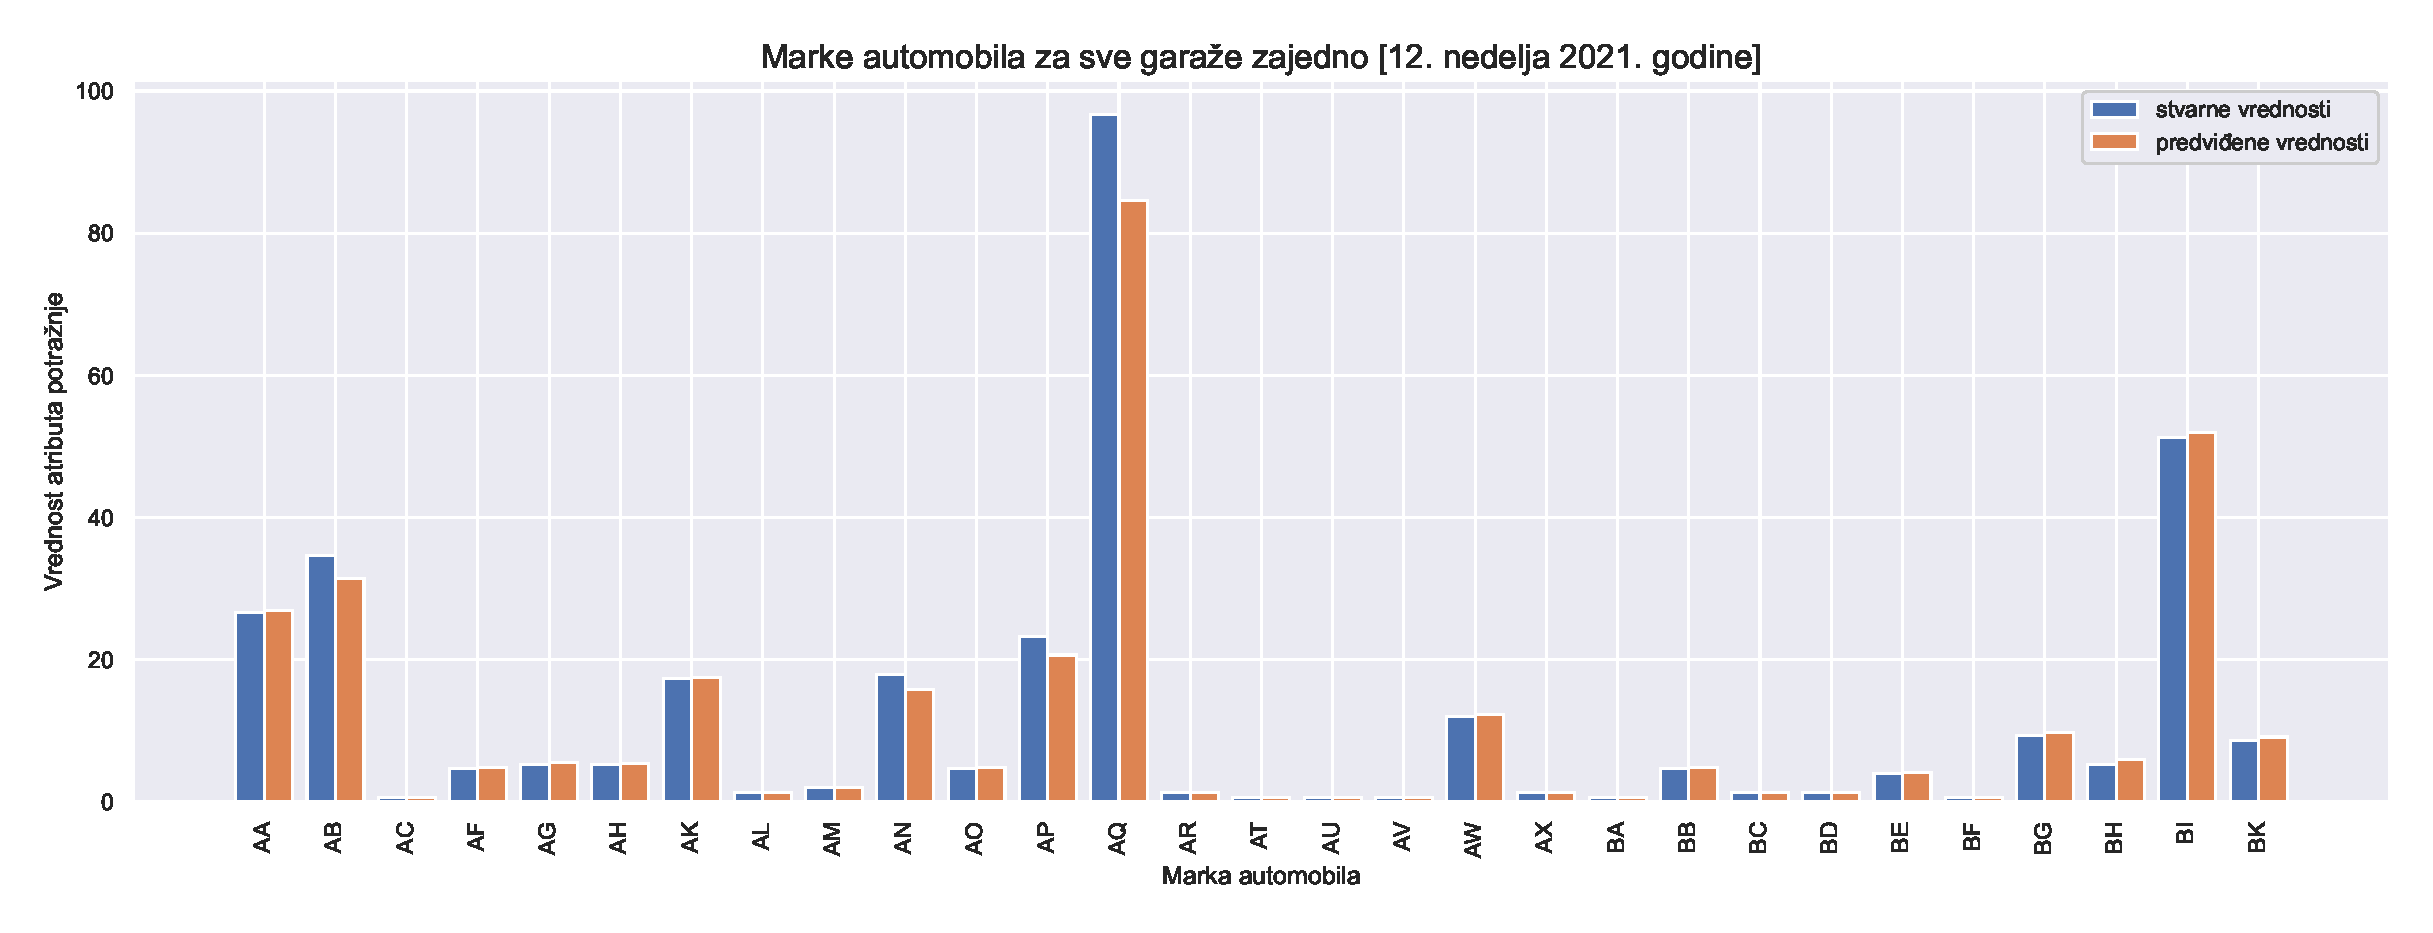
\includegraphics[width=1\textwidth]{./grafici/year_week_garage_make_train_on_all_available_202112.eps}
  \caption{Raspodela marki automobila za 12. nedelju 2021. godine} 
  \label{fig: marke_nedelja}
\end{figure}

\begin{figure}[!ht]
  \centering
  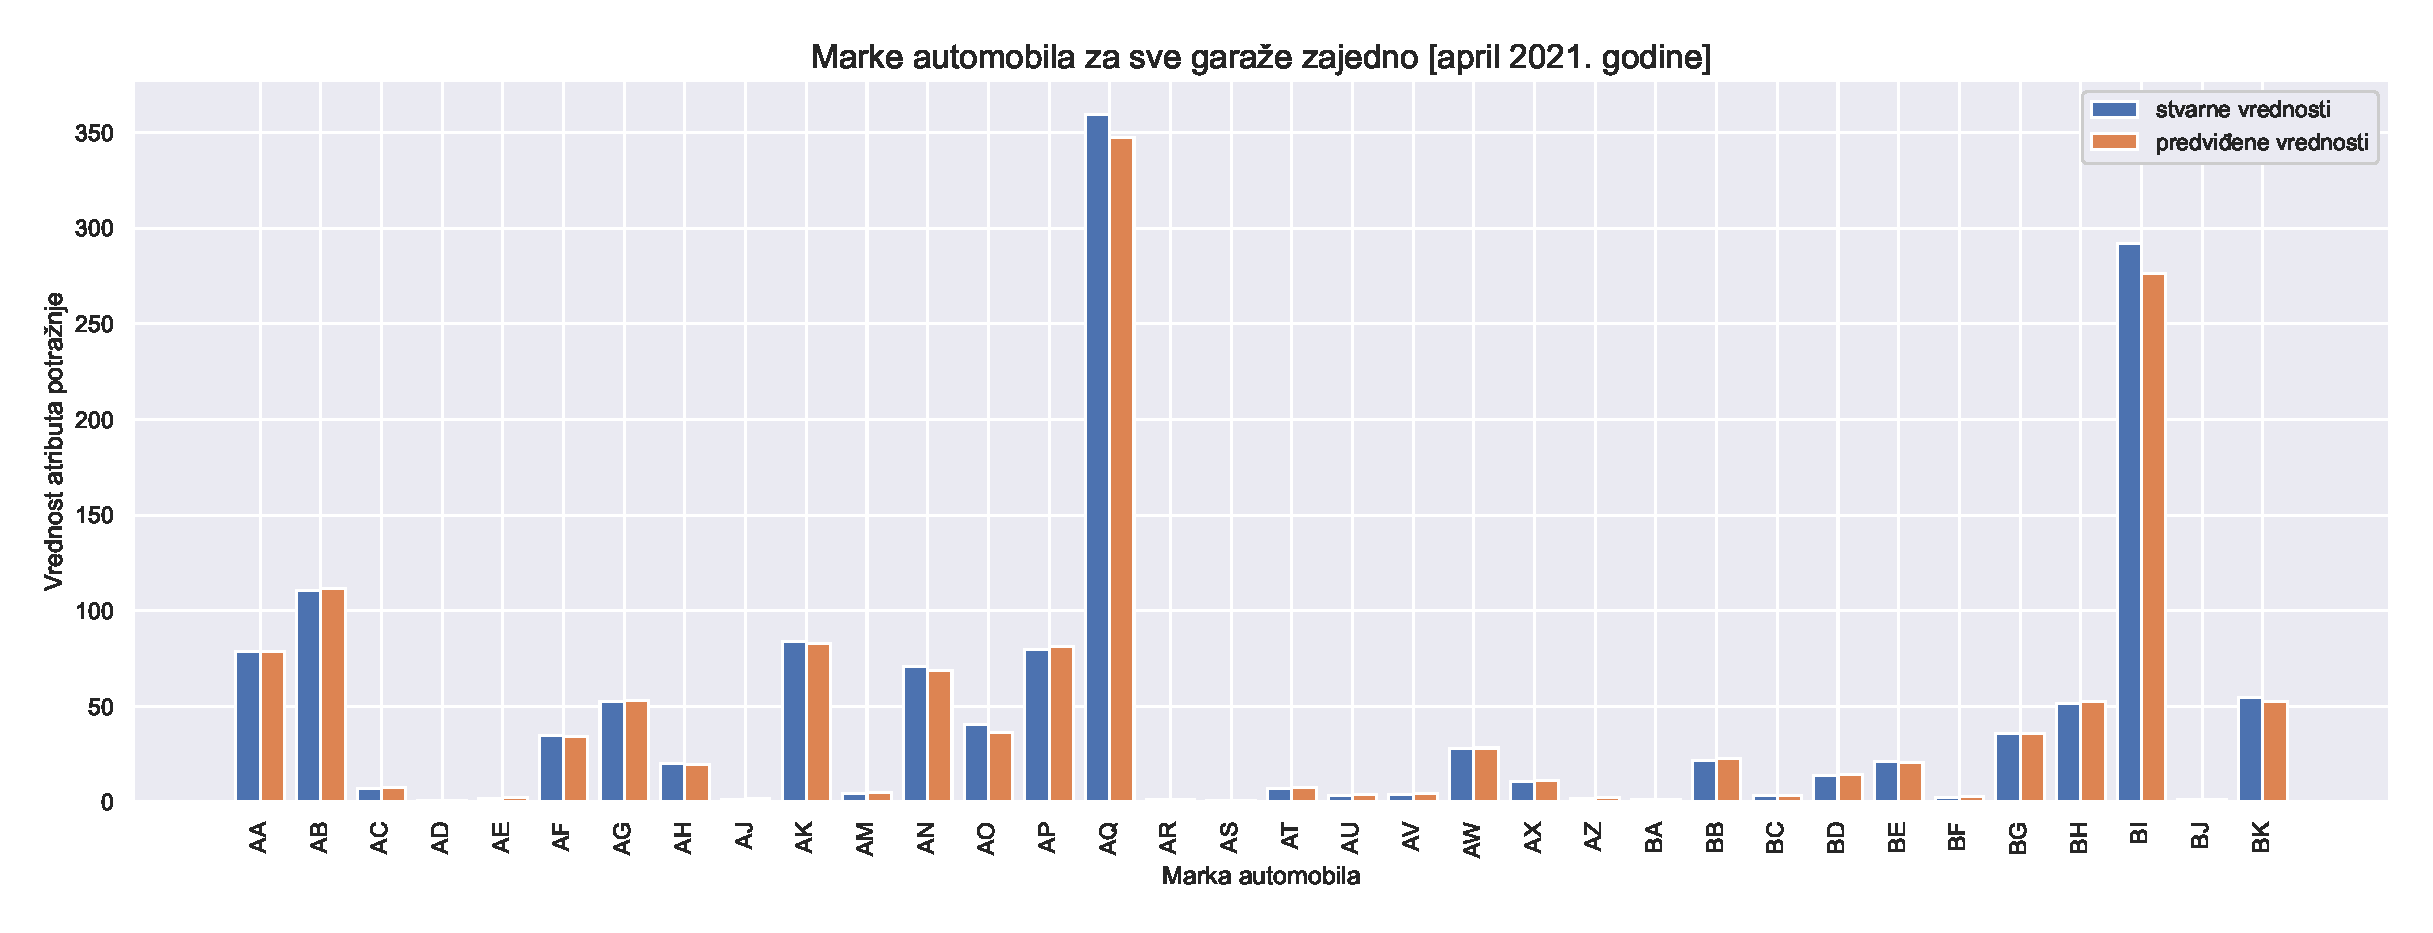
\includegraphics[width=1\textwidth]{./grafici/year_month_garage_make_train_on_all_available_202104.eps}
  \caption{Raspodela marki automobila za april mesec 2021. godine}
  \label{fig: marke_mesec}
\end{figure}

\section{Diskusija rezultata}
% ------------------------------------------------------------------------------
Izlaganje dato u prethodnim poglavljima doprinelo je da se bolje razumeju trenutno dostupni podaci. Otkriveno je da veliki broj automehaničarskih radnji spada u "manje" radnje, odnosno da mnoge od njih imaju veoma nisku vrednost ciljne promenljive \textit{demand\_value} koja je predviđana, ili je uopšte nemaju za dosta vremenskih trenutaka. To znači da je za problem vremenskih serija, grupisanje podataka na neki način bilo neophodno i da za posmatranje vremenskih serija za svaku automehaničarsku radnju po automobilskim markama još uvek nema značajan broj podataka.

Takođe, potrebno je da se novi izvor podataka (booking portal) sa kog su podaci i prikupljeni, još više aktivira kako bi reprezentacija podataka bolje predstavljala radnje ili da se podaci obogate i svim drugim izvorima podataka koji postoje za sve automehaničarske radnje (što je problem na kome se radi).

Dobra strana istraživanja vremenskih serija i XGBoost metoda na način na koji je posmatran za dnevne i nedeljne podatke, je da se vrednosti prethodnih dana/nedelja mogu ubaciti kao novi veštački atribut u skup atributa za predviđanje metodama mašinskog učenja, jer se pokazalo da postoji neki smisao ubacivanja vrednosti kašnjenja (vrednosti iz prošlosti), i da to može da doprinese modelu da uči. Broj vrednosti iz prošlosti bi mogao biti određen ARIMA modelima i njihovim koeficijentima.

Prophet je pre svega ispitivan zbog ideje da ima podršku da uračuna efekte praznika na uticaj modela. Kroz istraživanje se pokazalo da je bolje ubaciti efekte praznika i da oni mogu da imaju značajne efekte na model. Pre svega je grafik vremenske serije na nedeljnom nivou otkrio značajne padove oko nekih datuma koji potencijalno nastaju zbog praznika.

Uočena je i mana posmatranja problema kao sasvim regresionog kod XGBoost metode na većim granularnostima. Dolazak određene automobilske marke u neku automehaničarsku radionicu biva zabeležen i model se recimo obučava na takvim podacima, ali generalno regresioni problem neće da kaže da li je određena automobilska marka uopšte došla ili nije u automehaničarsku radnju. Dakle, potencijalno bi prvo trebalo uraditi binarnu klasifikaciju da je marka automobila došla ili nije došla, a zatim predviđati potražnju pomenute ciljne promenljive.

U tabeli \ref{tbl: sumarna_metrika} su predstavljene SMAPE vrednosti najboljih modela za dnevnu i nedeljnu vremensku seriju. Može se primetiti da se XGBoost ponaša najbolje u oba slučaja, jer je SMAPE vrednost najmanja za tu vrstu modela. ARIMA model na dnevnom nivou podataka daje najnepreciznija predviđanja i može se primetiti da su svi modeli na nedeljnom nivou približno jednako zadovoljavajući. 

\begin{table}[!ht]
\centering
\caption{Sumarna SMAPE metrika evaluacije za najbolje modele}
\label{tbl: sumarna_metrika}
\begin{tabular}{ |c|c|c|c|c|} 
\hline
IME MODELA & SMAPE DNEVNI & SMAPE NEDELJNI \\
\hline
ARIMA & 0.208 & 0.151\\
Prophet & 0.130 & 0.144\\ 
XGBoost & 0.127 & 0.139\\
\hline
\end{tabular}
\end{table}

\chapter{Zaključak i pravci daljeg rada}
% ------------------------------------------------------------------------------
Kao što je pomenuto u uvodnom delu, problem predviđanja potražnje je široko zastupljen problem. U automobilskoj industriji precizno predviđanje može da dovede do poboljšanja mnogih poslova, a samim tim i do uštede resursa, odnosno povećanja profita. Poslovi koji se mogu unaprediti u ovom konkretnom slučaju su naručivanja potrebne i dovoljne količine automobilskih delova, optimalnog distribuiranja tih delova do automehaničarskih radnji, pametno postavljanje popusta na popravke određenih automobilskih marki kako bi se povećali prihodi, a iskoristili neki zaostali delovi itd.

U ovom radu je opisan pristup za rešavanje novog problema koji je predstavljen od strane industrijskog sveta i stvarne kompanije. Rad nad realnim podacima je kao i uvek dosta izazovan, posebno u slučaju kada podataka ima jako malo i u ovom slučaju gde je situacija da je izvor za podatke krenuo sa radom kao nova ideja tek krajem 2019. godine. Nakon samog pokretanja desila se pandemija virusa i to je svakako uticalo da svi ovi dostupni podaci budu nestandardni -- što će biti interesantno istraživati u godinama koje tek dolaze, sa povećanjem količine podataka. Takođe, kada se prikupe i podaci iz drugih izvora koji su vezani za sve automehaničarske radnje, mogao bi da se ispita uticaj internet portala za rezervacije na globalnu sliku rada kompanije. Istraživanje je pokazalo da modeli mogu dobro da se ponašaju na grupisanom nivou (recimo nivou cele države) ili na nivou predviđanja velikih automehaničarskih radnji za koje postoje dovoljne količine podataka. Za male radnje postoji veliki problem sa nepostojećim informacijama vezanim za marke automobila, tako da bi možda neki drugi problem (klasifikacija+regresija) mogao da pomogne. Takođe, bitno je napomenuti da ono što je prema podacima sa veb portala za rezervacije mala ili velika radnja, ne mora da bude realna slika. To može da bude samo usled dostupnih podataka ili toga što se neka velika radnja tek skoro priključila ozbiljnijem korišćenju ovog načina rezervisanja popravki, pa deluje kao da je mala po količini ciljne promenljive (što se može nadomestiti dobijanjem pristupa drugim izvorima podataka u ovoj kompaniji).

Istraživanje je otvorilo i neke nove ideje. Pre svega sledeći korak bi mogao biti obogaćivanje trenutnih podataka podacima koji su javno dostupni, a vezani za vremensku prognozu. Moguće je za svaki vremenski trenutak i na osnovu lokacija automehaničarskih radnji dodati atribut koji bi predstavljao svojstva vremenske prognoze, kako bi se uočilo da li zima/leto imaju uticaj na to kada ljudi popravljaju svoje automobile. Kompanija poseduje informacije o svakom automobilu koji je bio na popravci (npr. godinu proizvodnje), tako da se za dalja istraživanja može gledati u pravcu obogaćivanja modela atributom poput trenutne približne cene automobila. Korišćenje Google Mapa umesto Open Street Mapa može doprineti preciznijem stanju, a možda i dobijanje javnih statističkih informacija o konkurentnim radnjama može da se uzme u obzir. Uzimanje više ličnih informacija korisnika ili više informacija o automobilima (pređena kilometraža, broj ukupnih vlasnika, broj oštećenja itd.) prilikom unosa rezervacije na veb portal, bi takođe moglo biti iskorišćeno u svrhe pravljenja boljih modela za predviđanja.

% ------------------------------------------------------------------------------
% Literatura
% ------------------------------------------------------------------------------
\literatura

% ==============================================================================
% Završni deo teze i prilozi
\backmatter
% ==============================================================================

% ------------------------------------------------------------------------------
% Biografija kandidata
\begin{biografija}

  \textbf{Anđelka Milovanović} je rođena u Valjevu 22. jula 1996. godine. Išla je u Osnovnu školu "Sestre Ilić" u Valjevu i u Muzičku školu "Živorad Grbić", odsek za flautu. Nakon završene osnovne škole, kao najbolji đak svoje generacije, upisala je specijalizovano-matematičko odeljenje u Valjevskoj gimnaziji. Paralelno sa gimnazijom, pohađala je srednju muzičku školu za flautu nekoliko meseci, dok se nije javilo interesovanje za neke druge oblasti. 
  
  Tokom srednje škole bila je polaznica seminara astronomije u Istraživačkoj stanici Petnica sve četiri godine i vodila je astronomsku grupu u Društvu istraživača "Vladimir Mandić -- Manda" u Valjevu. Organizovala je aktivnosti poput akcija za posmatranje meteorskih rojeva i drugih nebeskih objekata, pomračenja Sunca i Meseca, Sata za našu planetu, zimskih i letnjih astronomskih škola za učenike osnovnih i srednjih škola, raznih naučno-popularnih predavanja i mnoge druge. Fokus tokom srednje škole joj je uglavnom bio na vaannastavnim aktivnostima, tako da je bila jedan od organizatora prvog Festivala nauke u gimnaziji, volontirala je na događajima Centra za promociju nauke i učestvovala na Astro-vikendu u Domu Omladine Beograda. 
  
  Najinteresantnija oblast u srednjoj školi joj je bilo programiranje, tako da odlučuje da upiše smer Informatike na Matematičkom fakultetu u Beogradu. Nakon 2. godine fakulteta dobija punu stipendiju Američke Vlade za jednosemestralnu studentsku razmenu "Global UGRAD", na Univerzitetu na Floridi -- Florida Gulf Coast University. Nakon godinu dana pauze na Matematičkom fakultetu, vraća se svojim studijama. Osvojila je 1. mesto na međunarodnom hakatonu (TADHack 2019), u timu sa još dvojicom kolega. Iste godine je provela 1. semestar u ulozi studenta demonstratora na kursu Računarske grafike, a 2. semestar u ulozi praktikanta u Majkrosoft Razvojnom Centru Srbije (MDCS).    
  
  Nakon uspešno završenih osnovnih studija na Matematičkom fakultetu, Anđelka nastavlja obrazovanje i upisuje master studije na istom smeru. Iste godine dobija diplomu Društva istraživača, kao potvrdu velikog zalaganja za popularizaciju nauke i samog društva tokom srednjoškolskog perioda. 

\end{biografija}
% ------------------------------------------------------------------------------

\end{document}
